% Setup the document.
\documentclass[11pt]{report}


% Import packages used in the document.
\usepackage{latex_sty/mk-highlighting}
\usepackage{latex_sty/mk-annotated-ref}
\usepackage{latex_sty/er-tutorial}
\usepackage{latex_sty/er-abbrev}
\usepackage{latex_sty/er-math}
\usepackage{latex_sty/mk-enhanced-sampling}

\usepackage{upquote}
\usepackage[disable]{todonotes}

% Load any abbreviations.
% Abbreviations and command definitions.
\defineAbbreviation{CA}{cellular automata}
\defineAbbreviation{CET}{cryoelectron tomography}
\defineAbbreviation{CME}{chemical master equation}
\defineAbbreviation{CPU}{central processing unit}
\defineAbbreviation{CUDA}{Compute Unified Device Architecture}
\defineAbbreviation{DGL}{differential gene loss}
\defineAbbreviation{DS}{direct sampling}
\defineAbbreviation{ds-protein}{domain specific ribosomal protein}
\defineAbbreviationPlural{ds-protein}{ds-proteins}{domain specific ribosomal proteins}
\defineAbbreviation{EF-Tu}{elongation factor Tu}
\defineAbbreviation{EN}{extrinsic noise}
\defineAbbreviation{EP}{evolutionary profile}
\defineAbbreviation{ERM}{equal-rates Markov}
\defineAbbreviation{ES}{enhanced sampling}
\defineAbbreviation{FBA}{flux balance analysis}
\defineAbbreviation{FFPilot}{forward flux pilot sampling}
\defineAbbreviation{FPE}{Fokker-Planck equation}
\defineAbbreviation{GFP}{green fluorescent protein}
\defineAbbreviation{GPU}{graphics processing unit}
\defineAbbreviationPlural{GPU}{GPUs}{graphics processing units}
\defineAbbreviation{GRF}{gene regulation function}
\defineAbbreviation{GMP}{Gillespie multi-particle}
\defineAbbreviation{GTS}{genetic toggle switch}
\defineAbbreviation{HDFS}{Hadoop distributed file system}
\defineAbbreviation{HGT}{horizontal gene transfer}
\defineAbbreviation{HPC}{high performance computing}
\defineAbbreviation{IN}{intrinsic noise}
\defineAbbreviation{indel}{insertion or deletion}
\defineAbbreviationPlural{indel}{indels}{insertions or deletions}
\defineAbbreviation{IPTG}{isopropyl $\beta$-D-1-thiogalactopyranoside}
\defineAbbreviation{KL}{Kullback--Leibler}
\defineAbbreviation{LacI}{{\it lac} repressor}
\defineAbbreviation{LacY}{lactose permease}
\defineAbbreviation{LMES}{Lattice Microbes ES} 
\defineAbbreviation{LSU}{large subunit}
\defineAbbreviation{ME-EP}{maximum-entropy evolutionary profile}
\defineAbbreviation{MD}{molecular dynamics}
\defineAbbreviation{MFPT}{mean first passage time}
\defineAbbreviation{ML}{maximum-likelihood}
\defineAbbreviation{MPD}{mulitparticle diffusion}
\defineAbbreviation{MPD-RDME}{mulitparticle-diffusion RDME}
\defineAbbreviation{MR-RDME}{multiresolution RDME}
\defineAbbreviation{mRNA}{messenger RNA}
\defineAbbreviation{MSA}{multiple sequence alignment}
\defineAbbreviation{MSD}{mean square displacement}
\defineAbbreviation{MST}{mean switching time}
\defineAbbreviationPlural{MST}{MSTs}{mean switching times}
\defineAbbreviation{nm}{nanometers}
\defineAbbreviation{ns}{nanoseconds}
\defineAbbreviation{ODE}{ordinary differential equation}
\defineAbbreviationPlural{ODE}{ODEs}{ordinary differential equations}
\defineAbbreviation{OU}{Ornstein-Uhlenbeck}
\defineAbbreviation{PDE}{partial differential equation}
\defineAbbreviationPlural{PDE}{PDEs}{partial differential equations}
\defineAbbreviation{PDF}{probability density function}
\defineAbbreviationPlural{PDF}{PDFs}{probability density functions}
\defineAbbreviation{PFB}{positive feedback}
\defineAbbreviation{QBIO}{quantitative biology}
\defineAbbreviation{RBS}{ribosomal binding site}
\defineAbbreviation{RMSD}{root-mean-square deviation}
\defineAbbreviation{RNAP}{RNA polymerase}
\defineAbbreviation{REU}{Research Experiences for Undergraduates}
\defineAbbreviation{RDME}{reaction-diffusion master equation}
\defineAbbreviation{rRNA}{ribosomal RNA}
\defineAbbreviation{r-protein}{ribosomal protein}
\defineAbbreviationPlural{r-protein}{r-proteins}{ribosomal proteins}
\defineAbbreviation{SCT}{single-cell trap}
\defineAbbreviation{SSA}{stochastic simulation algorithm}
\defineAbbreviation{SSU}{small subunit}
\defineAbbreviation{SI}{supporting information}
\defineAbbreviation{SOQ}{Summer of QBIO}
\defineAbbreviation{SRG}{self-regulating gene}
\defineAbbreviation{SRP}{signal recognition particle}
\defineAbbreviation{TMG}{thiomethyl-$\beta$-D-galactoside}
\defineAbbreviation{TRN}{transcriptional regulatory network}
\defineAbbreviation{TOC}{table of contents}
\defineAbbreviation{UPT}{universal phylogenetic tree}
\defineAbbreviation{VM}{virtual machine}

% Species abbreviations.
\defineAbbreviationStrict{Ametal}{\textit{A. metalliredigens}}{\textit{Alkaliphilus metalliredigens}}
\defineAbbreviationStrict{Aorem}{\textit{A. oremlandii}}{\textit{Alkaliphilus oremlandii}}
\defineAbbreviationStrict{Bsubt}{\textit{B. subtilis}}{\textit{Bacillus subtilis}}
\defineAbbreviationStrict{Cacet}{\textit{C. acetobutylicum}}{\textit{Clostridium acetobutylicum}}
\defineAbbreviationStrict{Celegans}{\textit{C. elegans}}{\textit{Caenorhabditis elegans}}
\defineAbbreviationStrict{Cnovyi}{\textit{C. novyi}}{\textit{Clostridium novyi}}
\defineAbbreviationStrict{Dradio}{\textit{D. radiodurans}}{\textit{Deinococcus radiodurans}}
\defineAbbreviationStrict{Ecoli}{\textit{E. coli}}{\textit{Escherichia coli}}
\defineAbbreviationStrict{Fmagna}{\textit{F. magna}}{\textit{Finegoldia magna}}
\defineAbbreviationStrict{Hmaris}{\textit{H. marismortui}}{\textit{Haloarcula marismortui}}
\defineAbbreviationStrict{Lborg}{\textit{L. borgpetersenii}}{\textit{Leptospira borgpetersenii}}
\defineAbbreviationStrict{Mflag}{\textit{M. flagellatus}}{\textit{Methylobacillus flagellatus}}
\defineAbbreviationStrict{Mtuber}{\textit{M. tuberculosis}}{\textit{Mycobacterium tuberculosis}}
\defineAbbreviationStrict{Pingr}{\textit{P. ingrahamii}}{\textit{Psychromonas ingrahamii}}
\defineAbbreviationStrict{Saren}{\textit{S.  arenicola}}{\textit{Salinispora  arenicola}}
\defineAbbreviationStrict{Scerev}{\textit{S. cerevisiae}}{\textit{Saccharomyces cerevisiae}}
\defineAbbreviationStrict{Scoel}{\textit{S. coelicolor}}{\textit{Streptomyces coelicolor}}
\defineAbbreviationStrict{Ssolf}{\textit{S. solfataricus}}{\textit{Sulfolobus solfataricus}}
\defineAbbreviationStrict{Strop}{\textit{S. tropica}}{\textit{Salinispora tropica}}
\defineAbbreviationStrict{Ttherm}{\textit{T. thermophilus}}{\textit{Thermus thermophilus}}

% Grammar shortcuts.
\newcommand{\ie}{\textit{i.e.}\xspace}
\newcommand{\eg}{\textit{e.g.}\xspace}
\newcommand{\etal}{\textit{et al.}\xspace}

% Biology shortcuts.
\newcommand{\insitu}{\textit{in situ}\xspace}
\newcommand{\invivo}{\textit{in vivo}\xspace}
\newcommand{\invitro}{\textit{in vitro}\xspace}
\newcommand{\insilico}{\textit{in silico}\xspace}

% RDME definitions.
\newcommand{\xv}{{\vec{x}}}
\newcommand{\sv}{\vec{S}}
\newcommand{\rv}{\vec{r}}
\newcommand{\drv}{\vec{dr}}
\newcommand{\Dop}{{\mathcal D}}
\newcommand{\Rop}{{\mathcal R}}

% Unit shortcuts.
\newcommand{\Dunits}{$\mathrm{\mathsf{\mu m^2/s}}$\xspace}
\newcommand{\pMps}{$\mathrm{\mathsf{M^{-1} s^{-1}}}$\xspace}
\newcommand{\ps}{$\mathrm{\mathsf{s^{-1}}}$\xspace}
\newcommand{\uM}{$\mathrm{\mathsf{{\mu}M}}$\xspace}
\newcommand{\um}{$\mathrm{\mathsf{{\mu}m}}$\xspace}
\newcommand{\umcube}{$\mathrm{\mathsf{{\mu}m^3}}$\xspace}
\newcommand{\us}{$\mathrm{\mathsf{{\mu}s}}$\xspace}
\newcommand{\mmps}{$\mathrm{\mathsf{m^{2}\,s^{-1}}}$\xspace}
\newcommand{\umumps}{$\mathrm{\mathsf{{\mu}m^{2}\,s^{-1}}}$\xspace}

% Math shortcuts.
\newcommand{\nomath}[1]{$\mathrm{\mathsf{#1}}$\xspace}

% Custom macros.
\newcommand{\ROOT}{\code{\$FILES\_ROOT}\xspace}



% some top-level aliases shared amongst the chapters
\newcommand{\sbmlimport}{\noss{lm_sbml_import}}

% Start the document.
\begin{document}

%% Set the page numbering to be lowercase roman numerals for the front matter.
%\newpage
%\singlespacing
%\normalsize
%\setcounter{page}{1}
%%\renewcommand{\thepage}{\roman{page}}
%
%% Title page.
%\thispagestyle{empty}
%\begin{center}{
%\vspace*{0.85in}
%{\huge LMES Enhanced Sampling Guide}\\
%\vspace*{0.5in}
%{\large \today}\\
%\vspace*{0.9in}
%{\large Authors:}\\
%{\large Max Klein}\\
%~\\
%~\\
%{\large Roberts Group}\\
%{\large Johns Hopkins University}\\
%{\large \color{blue} \url{http://biophysics.jhu.edu/roberts/}}\\
%{\large \color{blue} \url{https://www.assembla.com/spaces/roberts-lab-public/wiki/Tutorials}}\\
%{\large \color{blue} \url{https://www.assembla.com/spaces/roberts-lab-public/wiki/LMES}}\\
%
%\vspace*{1.45in}
%{\Large Description}\\
%}\end{center}
%
%The ``LMES Enhanced Sampling Guide'' describes how to run and analyze simulations accelerated by enhanced sampling.
%
%~\\
%\begin{center}{
%{\Large System Requirements}\\
%}\end{center}
%This document assumes you will be using the latest LMES virtual machine image available from the LMES website. If you are using a different configuration, you may need to adjust the instructions in some places.

\setcounter{page}{132}

% Table of contents
\newpage
\tableofcontents

% List of tables
%\newpage
%\addcontentsline{toc}{chapter}{List of Tables}
%\listoftables

% List of figures
%\newpage
%\addcontentsline{toc}{chapter}{List of Figures}
%\listoffigures

% Set the page numbering to be arabic numerals for the text.
\newpage
\setcounter{chapter}{0}
%\setcounter{page}{1}
%\renewcommand{\thepage}{\arabic{page}}

% Main text.
\chapter{FFPilot simulation: conceptual overview}
\section{How to use FFPilot simulation}

\subsection{Use cases}

FFPilot can be used to greatly accelerate the simulation of a wide variety of systems. The primary use case for FFPilot is the simulation of systems with two (or more) well defined meta-stable states. With the correct setup, FFPilot will "ratchet" the simulation from one state to the other, yielding a great deal of information about the transition process and the probability landscape around and in-between the states.

In general, FFPilot should have a speed advantage over standard replicate simulation for any system that has a rough probability landscape with at least some large energetic barriers (equivalently, for any system encompassing rare events). 

\subsection{Non-use cases}

In theory, FFPilot simulation should be faster (in terms of internal simulation time) than replicate sampling in all cases. However, for certain types of systems the benefit of using FFPilot is expected to be minor:
\begin{description}[style=nextline]
    \item [$\bullet$ Systems with flat landscapes/no rare events]
    
        Systems in which the probability landscape is nearly flat, in that it lacks any significant barriers. In other words, systems with 0 fixed points.
    
    \item [$\bullet$ One-state systems]
    
        Systems that spend virtually all of their time in the neighborhood of a single point in their state space. In other words, systems with 1 fixed point.

\end{description}
For these types of systems replicate simulation will likely be faster (in terms of wall clock time) than FFPilot, due to various optimizations in the current version of Lattice Microbes. Thus, it is better to avoid the extra setup involved with using FFPilot when modeling these types of systems.

\section{FFPilot specific concepts}

FFPilot simulation is straightforward to set up, given that you at least know the rough locations (in terms of your system's state space) of the steady states of interest.

\subsection{Order parameters}

FFPilot uses an order parameter to distinguish one stable state from another, and to measure progress along a transition path. If FFPilot is thought of as driving a system from one state to another, then the order parameter defines the direction in which that driving occurs.

An order parameter is a function $\oparam: \left\{ \intnonnegs^\Speciescount \comma \realnonnegs \rightarrow \reals^\Oparamval \right\}$ of the species counts  and time of a system:
\begin{equation*}
    \oparamfunc{\speciescountx{0} \comma \cdots \comma \speciescountx{\Speciescount} \comma t} = \nseq{\oparamvalsymb}{\Oparamval}
\end{equation*}

An order parameters can thought of as a quantitative, mathematically defined version of a reaction coordinate.

\subsection{Tilings}
A tiling is a set of bins that spans the state space of a system. A tiling is defined in terms of an order parameter, a set of edges, and one or more initial basins (from which to start trajectories during phase zero). Multiple basins can be defined in order to carry out both forward and reverse simulation in a single run of \abr{LMES}.

Tilings can be defined in terms of a set of bin edges (also sometimes referred to as a set of interfaces). An FFPilot simulation will have as many 


- The edges are held in a 1D array called (appropriately enough) Edges.
- The initial basins are held in an N x D array called Basins, where N is the count of basins and D is the total number of unique chemical species in your system.
    - Each row in Basins represents a different basin, and each column in Basins holds the count of one particular chemical species in the model.
        - In other words, a basin is a single coordinate in the state space of the model.
    - Each initial basin should either be in front of the zeroth edge or behind the last edge.
        - Mathemtically, this means that one of $$ \mathscr{O}(\text{basin}) < \mathscr{O}(\text{Edges}[0]) $$ or $$ \mathscr{O}(\text{basin}) > \mathscr{O}(\text{Edges}[-1]) $$ should be true, where $\mathscr{O}$ is the order parameter of the tiling.

The rows in the `Basins` array determine where trajectories are started from during phase zero. A separate pilot and production stage (ie a whole separate FFPilot simulation) is run for each row in `Basins`. Thus, setting two different basins is a convenient way to run the simulations required to calculate the MFPT of both the forward switch (low A $\rightarrow$ high A) and the reverse switch (high A $\rightarrow$ low A) of the self regulating gene.

%\section{Error and error goal}
%An FFPilot simulation run at a 10\% error goal is mathematically guaranteed to produce MFPT estimates that are within 10\% of the true value 95\% (default value, this confidence level can be set as the user desires) of the time. This means that the MFPT estimates produced by two identical 10\% FFPilot simulations, or by the two symmetrical halves of a single 10\% error goal GTS simulation, should differ by no more than ${\sim}20\%$ relative to each other. However, FFPilot only directly controls for sampling error, so if there are other large sources of error

\chapter{Calculating values of interest from FFPilot output: theory}
\section{Mean first passage time}
The mean first passage time $MFPT_i$ to each edge $i$ of the tiling is calculated in terms of the weights $w_i$ as:
\begin{equation}
    MFPT_i = 
        \begin{cases}
            w_0 & \text{for}\ i=0, \\
            \\
            \frac{w_0}{\prod_{j=1}^{i} w_i} & \text{for}\ i>0.
        \end{cases}
\end{equation}
Thus, the overall $MFPT$ from the low A state to the high A state can be calculated as:
\begin{equation}\label{eq:mfpt_from_weights}
    MFPT = MFPT_N = \frac{w_0}{\prod_{j=1}^{N} w_i}.
\end{equation}
where N is the index of the final edge.

In terms of the phase weights $w_i$, the formula for the mean first passage time to the $j$th edge is:
\begin{equation*}
    \frac{w_0}{\prod_{i=1}^{j} w_i}.
\end{equation*}

\section{Landscapes produced by FFPilot}\label{sec:landscape_theory}

One of the primary goals of stochastic simulation of biological systems is to calculate the probability landscapes of those systems. For nonequilibrium steady-state systems, calculating the landscape is equivalent to solving the system's master equation. From it you can obtain complete information about the occupancies and fluxes of the system.

When working with FFPilot simulation output, the calculation of the complete unbiased probability landscape of a system can be thought of as the recursive process of building up larger histograms (in terms of the information content in each) from smaller ones. Of course the final, complete landscape is the primary interest, but the phase, stage, and transition region landscapes that you build in the process can be helpful for investigating the fine details of a system or of the simulation process itself.

\subsection{FFPilot phase landscapes}\label{sec:landscape_phase}
The first step in assembling the complete landscape hist is also the simplest. You just take the state samples collected during the FFPilot simulation and group them by phase. You then just bin them together into sparse histograms, one per phase run during a production stage.

\subsection{FFPilot stage landscapes}\label{sec:landscape_stage}
All of the phase $\ix>0$ hists (the phase 0 hists are dealt with later) are separated into groups based on their originating stage. Next, the phase hists in each group are combined via a simple weighted sum of their values. The weights, which we'll call the landscape weights $\landweight$, are calculated by the following piecewise formula:
\begin{equation}
\label{eq:landweight}
    \landweight =
    \begin{cases}
        \frac{1.0}{n_1} & \text{for}\ \ix=1, \\
        \\
        \frac{ \prod_{\jx=1}^{\ix - 1} w_{\jx}}{n_{\ix}} & \text{for}\ \ix>1,
    \end{cases}
\end{equation}
where $w_{\ix}$ is the phase $\ix$ weight and $n_{\ix}$ is the total count of trajectories run in phase $\ix$\footnote{\eqref{eq:landweight} only applies if you're taking state samples at a constant interval. Though discussion of a variable sampling time step is outside of the scope of this tutorial, the landscape weight formula can be modified\cite{Valeriani:2007hv} to allow for one.}.

The indices in \eqref{eq:landweight} are a bit confusing, so to give you a concrete example say that you ran a simulation that had 4 phases per stage. Phase 0 doesn't get a landscape weight, so your three $\landweight$ values would be:
\begin{align*}
    \landweightx{1} &= \frac{1.0}{n_1},\\
    \landweightx{2} &= \frac{w_1}{n_2},\\
    \landweightx{3} &= \frac{w_1 w_2}{n_3}.\\
\end{align*}



\subsubsection{The transition region and the span of the stage landscapes}
Due to the boundary conditions imposed in phases $\ix>0$, the stage hist will only cover the region of state space that was spanned by the tiling\footnote{Technically, what we mean by spanned region is all points $x$ in state space such that $\lambda_0 <= \oparam(x) < \lambda_N$} used to setup the FFPilot simulation. We will refer to this span as the transition region, since by construction it will lie in-between two (meta-)stable fixed points. The $\ix$th stage hist can be thought of as the conditional probability landscape of the transition region, given that the $\ix$th basin was the most recently visited. In other words, if a trajectory is in (or was most recently in) basin $\ix$, the $\ix$th stage hist will be effectively the instantaneous probability landscape for that trajectory.

%\subsection{Transition region landscape}\label{sec:landscape_transition}
%The stage hists calculated in the previous step are then weighted and combined into a single transition region hist. The stage weight factor $\stageweight$ of the $\mx$th stage is calculated as:
%\begin{itemize}
%    \item The flux across the initial interface $\ifacez$, which is calculated according to:
%    \begin{equation}
%        \Phi_{0|\mx} = \frac{\tau_{0|\mx}}{n_{0|\mx}^{s}} = \frac{1}{w_{0|\mx}}
%    \end{equation}
%which is the mean count of forward flux events per unit time during phase zero.
%    \item The \abr{MFPT}
%\end{itemize}
%
%\subsection{The complete unbiased landscape}\label{sec:landscape_complete}
%
%The last step of building up the landscape is also the most complicated one.  The protocol described here has proven robust across a variety of model system, but it is by no means guaranteed to work for every landscape.
%
%\section{The error goal, and how it relates to error in simulation outputs}
%
%\subsection{}
%
%\subsection{FFPilot }
%An FFPilot simulation run at a 10\% error goal is mathematically guaranteed to produce MFPT estimates that are within 10\% of the true value 95\% (default value, this confidence level can be set as the user desires) of the time. This means that the MFPT estimates produced by two identical 10\% FFPilot simulations, or by the two symmetrical halves of a single 10\% error goal GTS simulation, should differ by no more than ${\sim}20\%$ relative to each other. However, FFPilot only directly controls for sampling error, so if there are other large sources of error

{% enclose the chapter in braces to limit the scope of defined commands
\newcommand{\exampleroot}{\noss{notebooks}}
\newcommand{\srcdir}{\noss{\exampleroot\bs src}}
\newcommand{\srgname}{\noss{srg}}
\newcommand{\srgfullname}{\noss{self_regulating_gene}}
\newcommand{\srgmfpt}{\noss{{\srgname}_mfpt}}
\newcommand{\dir}{\noss{\exampleroot\bs\srgmfpt}}

\newcommand{\data}{data}
\newcommand{\dataw}{\noss{{\data}_worked}}
\newcommand{\sbml}{{\srgfullname}.sbml}
\newcommand{\lm}{\srgname.lm}
\newcommand{\out}{\noss{{\srgname}_out.sfile}}
\newcommand{\lmlog}{\srgname.log}
\newcommand{\nb}{\srgmfpt.ipynb}
\newcommand{\nbw}{\noss{{\srgmfpt}_worked.ipynb}}
\newcommand{\plotter}{plotTiling.py}

\newcommand{\datapath}{\dir\bs\data}
\newcommand{\datawpath}{\dir\bs\dataw}
\newcommand{\sbmlpath}{\exampleroot\bs{\sbml}}
\newcommand{\lmpath}{\datapath\bs\lm}
\newcommand{\outpath}{\datapath\bs\out}
\newcommand{\lmlogpath}{\datapath\bs\lmlog}
\newcommand{\nbpath}{\exampleroot\bs\nb}
\newcommand{\nbwpath}{\exampleroot\bs\nbw}
\newcommand{\plotterpath}{\srcdir\bs\plotter}

\newcommand{\lmpathrel}{\data\bs\lm}
\newcommand{\outpathrel}{\data\bs\out}
\newcommand{\lmlogpathrel}{\data\bs\lmlog}

\chapter{Using FFPilot to calculate mean first passage time (MFPT): self regulating gene}

\section{Overview}

In this section I'll go over how to use FFPilot to calculate the \abr{MFPT} of the \abr{SRG}. \abr{SRG} consists of a single protein, which I'll call protein A. Protein A participates in a positive feedback loop in which it upregulates its own production. Additionally, it experiences constant degradation. These properties make \abr{SRG} bistable, and it will stochastically switch from one state, with low levels of protein A, to another, with high levels of protein, and back again over time.

\begin{center}
    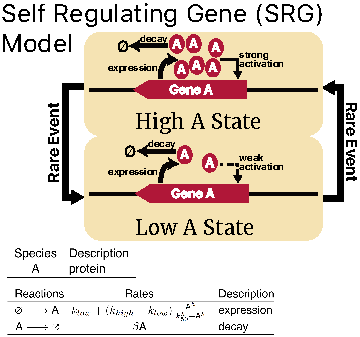
\includegraphics[width=5.0in]{{../Figures/model_schematics/self_regulating_gene}.pdf}
\end{center}

Starting from a \abr{SRG} model file included with this tutorial,\\
\pth{\sbmlpath}, I'll show you how to set up the simulation input file, execute the simulation, and analyze the output. If you execute the example commands and code exactly as written, you should end up with a new directory \pth{\datapath} that contains \pth{\lm}, the simulation input file, and \pth{\out}, the simulation output file. Pre-made example input and output files can be found in \pth{\datawpath}.

\section{Input file setup}\label{sec:srg_mfpt_input_setup}
The input file for an FFPilot simulation is the same as for standard (\ie direct sampling) simulation. However, some extra information is required, in the form of an order parameter and a tiling. %Input can be prepared in a few steps:
%\begin{enumerate}
%    \item Convert \pth{\sbml} $\rightarrow$ \pth{\lm}.
%    \item\label{item:add_op} Add an order parameter. 
%    \item\label{item:add_tiling_srg} Add a tiling.
%    \item\label{item:add_es_opts} Add any simulation options. 
%\end{enumerate}

\subsection{Convert .sbml -> .lm}\label{sec:sbml_conversion_srg}
Models of biochemical systems are often distributed in the SBML format. These can be converted to the \pth{.lm} format required by Lattice Microbes using the \pth{lm_sbml_import} utility.

Open a terminal and \sh{cd} to the \pth{\dir} directory. You will then execute the following commands:

\inputcmd{snippets/srg_mfpt/lm_sbml_import.sh}

The first command creates a separate \pth{\datapath} directory which we will use to hold any simulation input/output that we produce during this section of the tutorial. The last command converts \pth{\sbmlpath} file using  \pth{lm_sbml_import} and then places the resulting \pth{.lm} file at \pth{\lmpath}.

\subsection{Add an order parameter}\label{sec:add_op}
If fed into \abr{LMES} in its current form, \pth{\lm} could be used to run a standard replicate simulation. However, in order to use \pth{\lm} as input for an FFPilot simulation, we'll have to first open it up and add some extra information: an order parameter and a tiling. We'll start with the order parameter.

Internally, \pth{.lm} files are based on the \keyword{hdf5} format. This means that all of the existing \keyword{hdf5} software tools can directly interact with \pth{\lm}, just the same as for any \keyword{hdf5} file. We'll be using two of these \keyword{hdf5} tools in this tutorial:
\begin{description}[style=nextline]
    \item[\py{h5py}] A Python package that can open and/or modify \keyword{hdf5} files from within Python code. We'll be using \py{h5py} to modify the input file/add the extra information.
    \item[\exe{h5dump}] A command line tool that can be used to dump the contents of a \keyword{hdf5} file in plain text to the \keyword{stdout} of a terminal. We'll be using \exe{h5dump} to show the correct format for the extra input required by FFPilot.
\end{description}

The order parameter that we will use with \abr{SRG}, which I will call $\oparama$, will just be the count of the single chemical species in the system, protein A. Order parameter $\oparama$ is a linear combination of species counts and can thus be represented in \abr{LMES} as a linear order parameter. The following Python script will open up \pth{\lm} and add the definition of $\oparama$ in the required format:

\inputpy{snippets/srg_mfpt/add_order_parameter.py}

The above script adds a new group, \code{OrderParameters}, to \pth{\lm}, the contents of which we can inspect using \exe{h5dump} by opening a terminal, \pth{cd}-ing to \pth{\dir}, and then running the following command:

\inputcmd{snippets/srg_mfpt/h5dump_order_parameter.sh}

The dump will show that the \code{OrderParameters} group contains one subgroup, \code{0}:

\begin{minted}{text}
HDF5 "data/srg.lm" {
GROUP "OrderParameters" {
   GROUP "0" {
\end{minted}

Group \code{OrderParameters\bs0} contains the definition of $\oparama$. Two attributes are set on group \code{0}, \code{\oparamid} and \code{\oparamtype}:
\begin{minted}{text}
      ATTRIBUTE "ID" {
         DATATYPE  H5T_STD_I64LE
         DATASPACE  SCALAR
         DATA {
         (0): 0
         }
      }
      ATTRIBUTE "Type" {
         DATATYPE  H5T_STD_I64LE
         DATASPACE  SCALAR
         DATA {
         (0): 0
         }
      }
\end{minted}
These attributes, which are required in every order parameter definition, do the following:
\begin{description}[style=nextline]
    \item[\code{\oparamid}] This attribute (which should match the name of the \code{OrderParameters} subgroup on which it is set) is the name by which \abr{LMES} will refer to $\oparama$ internally.
    \item[\code{\oparamtype}] This attribute tells \abr{LMES} what kind of order parameter this is, and how it should interpret the order parameter's definition when calculating its value. A \code{\oparamtype} of \code{0} tells \abr{LMES} that $\oparama$ is a linear order parameter.
\end{description}

Inside of group \code{0} are two 1D arrays (by convention, \keyword{hdf5} tools refer to arrays as datasets), \code{\oparamspecids} and \code{\oparamcoeffs}:
\begin{minted}{text}
      DATASET "SpeciesCoefficients" {
         DATATYPE  H5T_IEEE_F64LE
         DATASPACE  SIMPLE { ( 1 ) / ( 1 ) }
         DATA {
         (0): 1
         }
      }
      DATASET "SpeciesIDs" {
         DATATYPE  H5T_STD_I64LE
         DATASPACE  SIMPLE { ( 1 ) / ( 1 ) }
         DATA {
         (0): 0
         }
      }
\end{minted}
\abr{LMES} uses the values in these arrays to define the formula for the value of an order parameter. For any linear order parameter $\oparam$, \abr{LMES} will use the following formula to calculate its value:
\begin{equation}
\label{eq:oparam_linear}
    \oparam = \sum_{\ix=0}^{\mcode{len(\oparamspecids)} - 1} \mcode{\counts[\oparamspecids[i]]} * \mcode{\oparamcoeffs[i]}
\end{equation}
where \code{\counts} is a 1D array containing the present count of each species in the system being simulated. \eqref{eq:oparam_linear} can be simplified considerably for $\oparama$:
\begin{align}
    \oparama &= \mcode{\counts[\oparamspecids[0]]} * \mcode{\oparamcoeffs[0]} \nonumber \\
    \oparama &= \mcode{\counts[0]} * \mcode{1} \nonumber \\
    \oparama &= \mcode{\counts[0]} \nonumber
\end{align}

\subsection{Add a tiling}\label{sec:add_tiling_srg}
Now we add a tiling to the self regulating gene. The tiling will be defined in terms of order parameter $\oparama$. In the previous section we added $\oparama$ to \pth{\lm} and gave it an \code{ID} of \code{0}. The following Python script will open up \pth{\lm} and add a new tiling with an \code{ID} of \code{0}:

\inputpy{snippets/srg_mfpt/add_tiling.py}

Once the script has run, we can inspect the contents of the newly added \code{Tilings} group in \pth{\lm} by opening a terminal, \sh{cd}-ing to \pth{\dir}, and then running the following command:

\inputcmd{snippets/srg_mfpt/h5dump_tiling.sh}

The dump shows one subgroup, \code{0}, in the \code{Tilings} group:
\begin{minted}{text}
HDF5 "data/srg.lm" {
GROUP "Tilings" {
   GROUP "0" {
\end{minted}

Group \code{Tilings\bs0} has three required attributes set on it:
\begin{minted}{text}
      ATTRIBUTE "ID" {
         DATATYPE  H5T_STD_I64LE
         DATASPACE  SCALAR
         DATA {
         (0): 0
         }
      }
      ATTRIBUTE "OrderParameterID" {
         DATATYPE  H5T_STD_I64LE
         DATASPACE  SCALAR
         DATA {
         (0): 0
         }
      }
      ATTRIBUTE "Type" {
         DATATYPE  H5T_STD_I64LE
         DATASPACE  SCALAR
         DATA {
         (0): 0
         }
      }
\end{minted}
the description of which are as follows:
\begin{description}[style=nextline]
    \item[\code{\tilingid}] This attribute (which should match the name of the \code{Tiling} subgroup on which it is set) is the name by which \abr{LMES} will refer to this tiling internally.
    \item[\code{\tilingtype}] A tiling \code{\tilingtype} of \code{0} tells \abr{LMES} that this is a 1D linear tiling\footnote{1D linear is the only kind of tiling currently implemented in \abr{LMES}. Thus, for now, this is just a placeholder value that should always be set to 0. In the future, more complex tilings, such as ones based on the Voronoi tessellation\cite{Dickson:2009gt}, may be implemented.}.
    \item[\code{\tilingopid}] The \code{\oparamid} of the order parameter (in this case, $\oparama$) that will be used in the definition of this tiling. Specifically, the placement of the edges that separate the tiles/bins of this tiling will be specified in terms of the tiling's order parameter.
\end{description}

Inside of group \code{Tilings/0} are a 2D array, \code{\tilingbasins}, and a 1D array, \code{\tilingedges}:
\begin{minted}{text}
      DATASET "Basins" {
         DATATYPE  H5T_STD_I64LE
         DATASPACE  SIMPLE { ( 2, 1 ) / ( 2, 1 ) }
         DATA {
         (0,0): 10,
         (1,0): 160
         }
      }
      DATASET "Edges" {
         DATATYPE  H5T_IEEE_F64LE
         DATASPACE  SIMPLE { ( 13 ) / ( 13 ) }
         DATA {
         (0): 23, 33.5833, 44.1667, 54.75, 65.3333, 75.9167, 86.5, 97.0833,
         (8): 107.667, 118.25, 128.833, 139.417, 150
         }
      }
\end{minted}
These arrays are used in the following way:
\begin{description}[style=nextline]
    \item[\code{\tilingedges}] Each entry in this array holds a single coordinate given in terms of the tiling's order parameter. \abr{LMES} builds up a tiling by placing edges at these coordinates. In turn, the tiles/bins themselves are defined as the space in between any two adjacent edges. The size of the \code{\tilingedges} array is directly related to the number of separate phases run during an FFPilot simulation. During each stage there will be exactly as many phases executed as there are edges in the tiling used to set up the stage.
    \item[\code{\tilingbasins}] An N x D array, where N is the count of basins and D is the total number of unique chemical species in your system. The basins (which are defined in terms of a model's complete state space) are the points in the state space of a system from which the initial trajectories of each stage (\ie the phase zero trajectories) will be launched. Each row in \code{\tilingbasins} is treated as a separate basin.
\end{description}

The rows in the \code{\tilingbasins} array determine where trajectories are started from during phase zero. One complete self-contained FFPilot simulation (\ie a pilot stage following by a production stage) will be executed for each basin specified in the simulation input's tiling. Thus, setting two different basins is a convenient way to run the simulations required to calculate the \abr{MFPT} of both the forward switch (low A $\rightarrow$ high A) and the reverse switch (high A $\rightarrow$ low A) of the \abr{SRG} model.

The Python script we used to create our tiling will have set up two basins. The initial basin is at 10 counts of protein A, corresponding to the low A state of \abr{SRG}. This is located in front of the zeroth edge of tiling (which sits at 23 counts of A). The other basin is at 160 counts of protein A, corresponding to the high A state of \abr{SRG}. This basin is located behind the last edge of the tiling (which sits at 150 counts of A). The following figure gives a sense of what the tiling actually looks like:

\begin{center}
    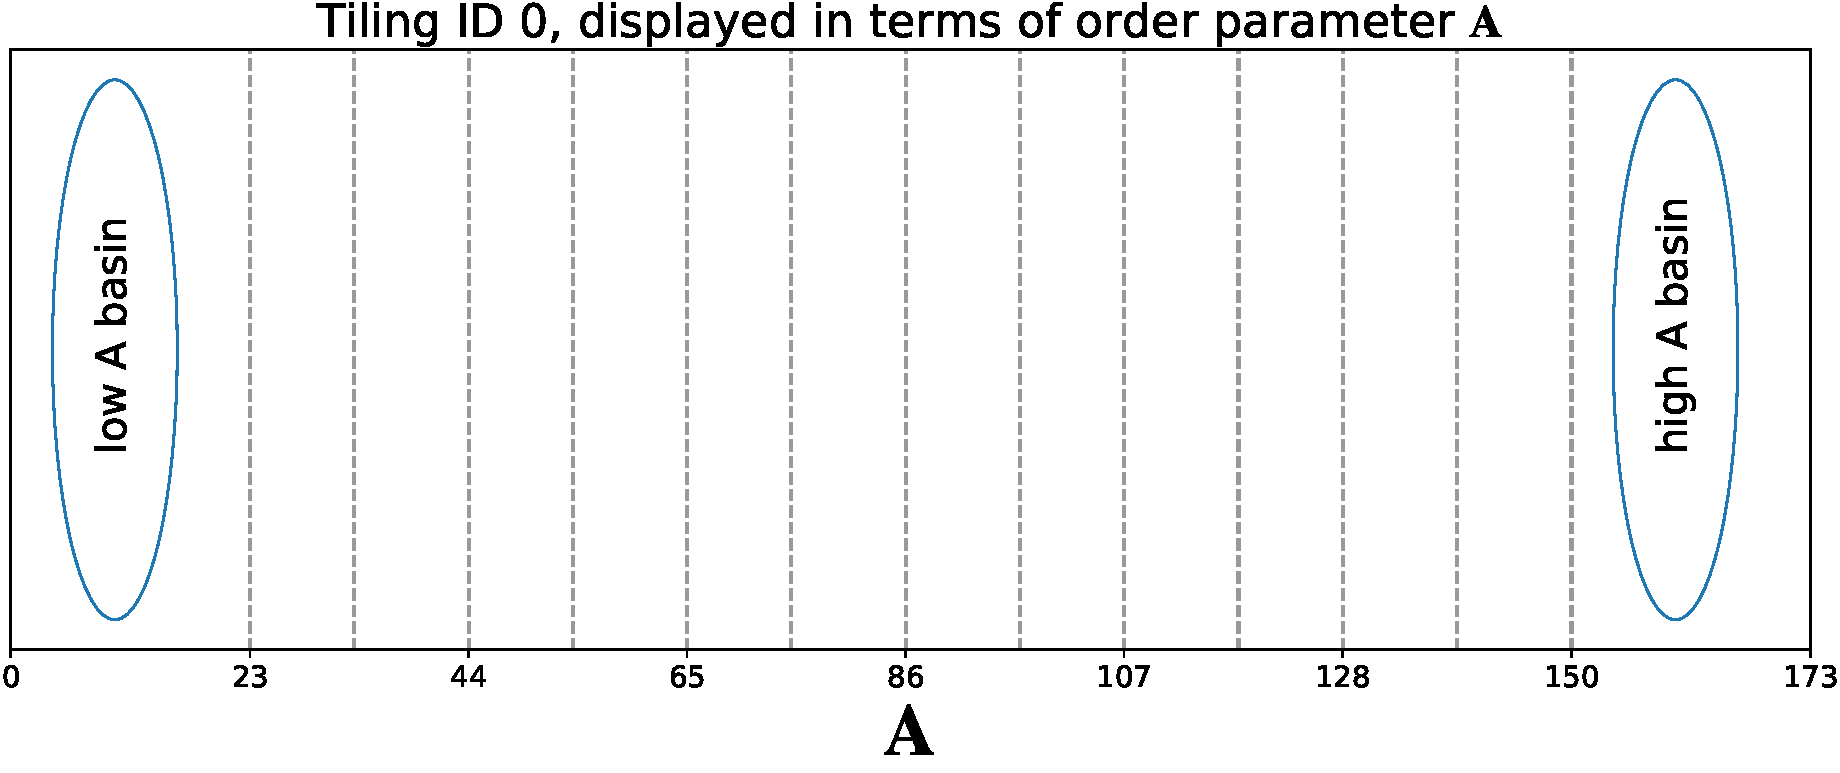
\includegraphics[width=6.0in]{{../Figures/srg_edges}.pdf}
\end{center}

\subsection{(advanced) FFPilot batch mode (multiple tilings)}

In normal usage, the input file for an FFPilot simulation should have exactly one tiling. However, FFPilot simulations can be run in large batches by specifying multiple tilings. In this case, each separate tiling will be treated as if it describes a separate simulation. In other words, an FFPilot simulation run using an input that contains M separate tilings is equivalent to running a batch of M separate FFPilot simulations.

NB: when creating an input file to use with FFPilot batch mode, each tiling should have its own unique \code{ID}.

\subsection{Customize FFPilot simulation options}\label{sec:customize_opts_srg}

FFPilot is designed to require as little user input as possible. All of the simulation options/parameters that FFPilot uses have reasonable (and, in some cases, adaptive) default values. On the other hand, FFPilot supports a number of options that can be used to control many different aspects of the simulation. In \pth{.lm} input files, options are set as attributes on the top level \code{Parameters} group. 

NB: \pth{lmes} only recognizes options set with values of type \code{str}. All non-string options (\ie \code{int}, \code{bool}, etc.) should be converted to \code{str} before they are set.

We'll set up some options for our FFPilot \abr{SRG} simulation using the following python script (which contains several examples of \code{str} conversion):

\inputpy{snippets/srg_mfpt/add_options.py}

In the above script, we set three options:
\begin{description}[style=nextline]
    \item[\code{ffluxPilotOutput}] \code{bool}, defaults to \code{False}. Turns on output of records from any pilot stages run during the simulation. Normally only simulation output from the production stages is saved, and the data from every pilot stage is discarded once its corresponding production stage has been set up. When this flag is set to \code{True}, however, output from both the pilot and the production stages is saved.
    \item[\code{errorGoal}] Percentage, specified as a \code{float} in the range \code{(0-1.0]}, defaults to \code{.05}. Sets a goal for the (percent) error in the overall basin-to-basin \abr{MFPT} calculated by each production stage. Based on the outcome of the preceding pilot stage, FFPilot automatically determines how many trajectories to launch in each phase of a production stage in order to achieve a sampling error at or below the set error goal. Set \code{errorGoal} to \code{.01} for a high accuracy simulation, or set it to \code{.10}+ for a relatively fast simulation.
\end{description}

\section{Running the simulation}\label{sec:running_srg_mfpt}
Now that the FFPilot input is prepared, you can execute the simulation by opening a terminal, \pth{cd}-ing to \pth{\dir}, and entering the following command:

\inputcmd{snippets/srg_mfpt/lmes.sh}

As shown above, running an FFPilot simulation requires two flags to be passed to the \abr{LMES} executable:
\begin{description}[style=nextline]
    \item[\code{-ffpilot}] Tells \abr{LMES} to run in FFPilot mode. Without this flag a default replicate simulation would be run instead.
    \item[\code{-f <input-path>}] Tells \abr{LMES} that the simulation input file can be found at \code{<input-path>}.
\end{description}

The path at which the simulation output will be saved is automatically determined from the input path. In this case, that means the simulation output will be saved to\\
\pth{\outpathrel}. Alternatively, you can explicitly set the simulation output path by specifying the \code{-fo <output-path>} flag on the command line when you execute \abr{LMES}.

Since this simulation is set up using a relatively loose 10\% error goal, it should run to completion fairly quickly. When run on my laptop (3.1 GHz, 4 CPU cores), the simulation finishes in about 30 seconds.

\subsection{(advanced) Preserving the simulation log}
Normally, the \pth{lmes} simulation log gets dumped directly to the terminal as the simulation runs. You can instead preserve the log for later perusal by running \pth{lmes} with a slightly modified command:

\inputcmd{snippets/srg_mfpt/lmes_log.sh}

where we've saved the simulation log to \pth{\lmlogpath} using \sh{>}, the Linux redirection operator.

One downside of redirecting the log is that it will prevent any progress messages from getting printed out to the terminal, making it hard to tell if the simulation is running correctly. One workaround is to monitor the log file in real time using the \code{watch} command while the simulation adds to it:

\inputcmd{snippets/srg_mfpt/watch_log.sh}

where the \code{-n} flag controls the number of lines that are displayed.

\section{Analyzing the log}

As an \pth{lmes} simulation runs, an informative log is dumped to \pth{stdout}. Aside from helping to monitor simulation progress, a large quantity of information about the outcome of an FFPilot simulation can be gleaned from the simulation log alone. For example, the \abr{MFPT} estimate is printed out at the end of every stage, eliminating the need to dig around in the actual simulation output file for this value. As well, the log contains some unique metadata about the simulation, such as the total elapsed wall-clock time.
% \footnote{Do not be concerned if the lines of the log get printed on top of each other, or if a particular log message is printed out more than once. These behaviors are by design, and are not indicative of bugs in the simulation.}

\subsection{FFPilot simulation progress log messages}

FFPilot simulations, like all \pth{lmes} simulations, begin with a kickoff phase, during which input is parsed and all of the parallel processes are initialized and coordinated. Once the kickoff is complete (usually only a few seconds when running \pth{lmes} on a single computer), an FFPilot simulation begins in earnest with the start of the pilot stage, as signaled by the following line getting printed to the log:
\begin{minted}{text}
Forward Flux stage 0 started (tiling_id: 0, basin_id: 0, stage_type: Pilot)
\end{minted}
This type of progress message is printed out at the start of every simulation stage. Each comma-separated term in between the parentheses holds a piece of information about the current simulation stage:
\begin{description}[style=nextline]
    \item[\code{tiling_id}] This gives the \code{ID} of the tiling used to set up the simulation stage. This matches the \code{ID} of the tiling we created earlier (see \secref{sec:add_tiling_srg}), and confirms that it was used to set up this simulation stage.
    \item[\code{basin_id}] This corresponds to the row index of \code{\tilingbasins} from which the basin species counts for this stage were taken. These basin species counts will be used to initialize phase 0 trajectories during this stage.
    \item[\code{stage_type}] Tells you whether this is a pilot or a production stage. One of each kind of stage is run for each basin in each tiling present in the simulation input.
\end{description}

Another kind of progress message is printed out at the start of each phase zero:
\begin{minted}{text}
Forward Flux phase 0 started (zeroth_edge: 23.00, \
    phase_limit: FORWARD_FLUXES >= 10000.00)
\end{minted}
The terms in the parentheses give some information about how this phase will be executed:
\begin{description}[style=nextline]
    \item[\code{zeroth_edge}] The coordinate of the tiling edge (given in terms of the tiling's order parameter) closest to the basin in which this phase's trajectories are initialized. Each time a phase zero trajectory crosses the \code{zeroth_edge} while traveling away from its starting basin, the simulation counts this as a single forward flux event. Additionally, the state that the trajectory was in when it fluxed forward is added to the dictionary of starting states that will be used to initialize trajectories during phase 1.
    \item[\code{phase_limit}] Describes the condition that must be fulfilled in order for this phase to be considered complete. This particular \code{phase_limit} means that 10,000 forward flux events (summed across all phase zero trajectories) need to be observed before this phase will be terminated. Phase zero is always run using a \code{FORWARD_FLUXES} type \code{phase_limit}.
\end{description}

A slightly different progress message is printed out at the start of each phase $i>0$:
\begin{minted}{text}
Forward Flux phase 4 started (starting_edge: 54.75, goal_edge: 65.33, \
    phase_limit: FORWARD_FLUXES >= 10000.00)
\end{minted}
where the values in the parentheses mean:
\begin{description}[style=nextline]
    \item[\code{starting_edge}] The edge along which lies all of the starting states used to initialize trajectories during this stage.
    \item[\code{goal_edge}] Once a trajectory has been launched from \code{starting_edge} it will continue to run until it either crosses the \code{zeroth_edge} (as specified in the most recent phase zero progress message) or this \code{goal_edge}. In either case the simulation is immediately terminated. However, if the trajectory was stopped because it crossed the \code{goal_edge}, the simulation counts this as a forward flux event. As well, the state the trajectory was in when it fluxed forward is added to the dictionary of starting states that will be used to initialize trajectories in the next phase.
\end{description}
The \code{phase_limit} term means the same thing in the phases $i>0$ progress messages as it does in the phase zero progress message. However, unlike phase zero, the type of \code{phase_limit} used to run any given phase $i>0$ varies depending on whether the phase is part of a pilot or a production stage. Essentially, the type of the \code{phase_limit} determines the phase's termination condition:
\begin{description}[style=nextline]
    \item[\code{FORWARD_FLUXES >= n}] 
    The type of \code{phase_limit} used during pilot stages. Each phase $i>0$ will only be considered complete once \code{n} forward flux events (\ie the count of trajectories that reached the \code{goal_edge}) have been observed, regardless of how many trajectories have been launched in total.
    \item[\code{TRAJECTORY_COUNT >= n}] 
    The type of \code{phase_limit} used during production stages. Each phase $i>0$ is considered complete once the total number of trajectories that have been launched and run to termination is \code{n}.
\end{description}

\subsection{Stage outcome log messages}

Every time a pilot stage finishes, some of the highlights from its output are added to the log file:
\begin{minted}{text}
The phase costs are:
[4.62, 0.151, 1.61, 2.41, 2.72, 2.09, 1.65, 1.22, 0.967, 1.01, 0.951, \
    1.25, 1.5]
The phase weight sample variances are:
[152, 0.018, 0.12, 0.228, 0.245, 0.155, 0.0665, 0.0211, 0.00473, 0.00296, \
    0.000693, 0.000495, 0.000396]
Conservative estimates of the phase weights are:
[4.62, 0.0179, 0.137, 0.345, 0.56, 0.8, 0.922, 0.974, 0.993, 0.995, 0.998, \
    0.998, 0.999]
Attempting to achieve error goal 0.05 (confidence level 0.95) \
    with the following optimized trajectory counts:
[32385, 497266, 51746, 23142, 14016, 9022, 5917, 3830, 2210, 1792, 1148, \
    1000, 1000]
\end{minted}
\begin{description}[style=nextline]
    \item[phase costs] The $i$th entry of this array holds the average cost, in terms of the internal simulation time, of collecting a single sample (\ie observation of a forward flux event) during phase $i$.  
    \item[variances] The $i$th entry of this array holds the variance of the samples collected during phase $i$. The samples in question are used to estimate the phase weights at the end of each phase.
    \item[conservative weight estimates] The $i$th entry of this array holds the estimate of phase weight $i$ that is calculated at the end of each phase $i$.  of the samples collected during phase $i$.
\end{description}

The values in these first 3 arrays are used to parameterize the FFPilot optimizing equation\todo{add ref to my paper in submission}. The FFPilot optimizing is used to predict the optimal simulation plan (\ie count of trajectories to launch in each phase) for the upcoming production stage. By optimal, I mean the simulation plan that will achieve the specified error goal with the least computational effort possible. 

The reason why the weight estimates shown above are referred to as "conservative" is that, following their initial calculation, they have each been run through a set of biased estimators. These biased estimators have been designed such that when the conservative weight estimates are used to parameterize the FFPilot optimizing equation, the optimizing equation is in turn slightly biased towards overestimating the number of trajectories required to achieve the error goal. This has the beneficial effect of helping to ensure overall simulation accuracy, albeit at a small cost in computational efficiency. 

The last array in the pilot stage output log message contains the prediction of the FFPilot optimizing equation, given the values in the first 3 arrays:
\begin{description}[style=nextline]
    \item[optimized trajectory counts]
    The trajectory counts in this array are used to set up the \code{phase_limits} during the pilot stage. In other words, each phase $i>0$ of the production stage will be run until the count of trajectories that have run to completion reaches \\
    \code{optimized_trajectory_counts[i]}.
\end{description}

Each production stage also adds some the highlights from its results to the log once it finishes:
\begin{minted}{text}
The phase costs are:
[4.72, 0.151, 1.58, 2.42, 2.71, 2.08, 1.66, 1.28, 1.02, 1.03, 0.974, \
    1.24, 1.49]
The phase weights are:
[4.72, 0.0186, 0.145, 0.353, 0.573, 0.814, 0.926, 0.977, 0.993, 0.998, \
    1, 1, 1]
The first passage times to each tile edge are:
[4.72, 254, 1.76e+03, 4.97e+03, 8.67e+03, 1.07e+04, 1.15e+04, 1.18e+04, \
    1.19e+04, 1.19e+04, 1.19e+04, 1.19e+04, 1.19e+04]
The overall first passage time from the starting basin to the \
    last tile edge is:
1.19e+04
\end{minted}

\begin{description}[style=nextline]
    \item[phase costs and weights]
    Same as from the pilot stage, but produced by the more accurate production stage.
    \item[mean first passage times] The $i$th entry in this array is the expected value of the time it takes to get from the simulation's starting basin to the $i$th edge of the tiling.
    \item[overall mean first passage time] The expected value of the time it takes to get from the simulation's starting basin to the ending basin. Equivalent to the final entry in the \abr{MFPT} array printed above. The basins can be thought of as the metastable states of the system, so the overall \abr{MFPT} can also be thought of as the inverse of the switching rate between those states.
\end{description}

\section{Browsing FFPilot output with dumpSFile}

Output from an FFPilot simulation takes the form of an \keyword{SFile}. By default, given that your simulation input is named \pth{<fname>.lm} the output is saved to \pth{<fname>_-_out.sfile} (this can be overridden by setting the \code{-fo <output-name>} cmd line option when running \abr{LMES}). \keyword{SFile} is a binary file format that holds information in the form of records. Each record begins with a short metadata section (record name, record type, data size in bytes) followed by a data section. For \abr{LMES} output in the \keyword{SFile} format, the data section takes the form of a serialized \href{https://developers.google.com/protocol-buffers/}{protocol buffer} message.

Although \keyword{SFiles} are not human readable, the \exe{dumpSFile} tool provided by the \code{robertslab} Python package can be used to easily view the contents of any \keyword{SFile}. For each record in an \keyword{SFile}, \exe{dumpSFile} converts the metadata into a human readable format, deserializes and formats the data portion, and then prints the results to \code{stdout}. The following command will dump the entire contents of \pth{\outpathrel} to the terminal:

\inputcmd{snippets/srg_mfpt/dump_all.sh}

The output will look something like this:

\inputout[fontsize=\tiny]{snippets/srg_mfpt/dump_all.txt}

The reason why the short simulation we just ran produced so much data is that we had turned on extra output via the \code{ffluxPilotOutput} option\footnote{If the simulation had been run using the default output options, the output would contain only 2 records, the summaries from each of the production stages.}. 

For each record it finds, \exe{dumpSFile} will first print out a line containing the record's metadata. This metadata has the following format:
\begin{minted}{text}
record.name    record.dataType    record.dataSize
\end{minted}
The data section of the record will then be printed out starting on the next line after the metadata.

\exe{dumpSFile} has many options that can help to tame the torrent of data. Here's a couple of the more useful ones:
\begin{description}[style=nextline]
    \item[\code{-i/--include <pattern0> <pattern1> ...}]
        When this option is set, \exe{dumpSFile} will attempt to match each regular expression \code{<patterni>} to each record. Records will only be printed out if  every pattern matches either the record's \code{name} or its \code{dataType}. Otherwise, \exe{dumpSFile} will skip the record. Patterns passed to \code{-i} are case insensitive.
        
        For example, the following \exe{dumpSFile} command, which passes the terms "summary", \\"production", and "basins/1"  to the \code{-i} flag:
        
        \inputcmd[fontsize=\footnotesize]{snippets/srg_mfpt/dump_include.sh}
        
        The "basins/1" and "production" terms match to \code{record.name}, and the "summary" term matches to \code{record.dataType}. This limits output to a single stage summary record, the one from the production stage that was initialized in basin \code{ID} \code{0}:
        
        \inputout[fontsize=\tiny]{snippets/srg_mfpt/dump_include.txt}
    
    \item[\code{-e/--exclude <pattern0> <pattern1> ...}]
        The opposite of \code{-i/--include}. Records will be excluded if every \code{<patterni>} matches either its \code{name} or its \code{dataType}.
    
    \item[\code{-l/--list-only}]
        When this flag is passed to \exe{dumpSFile}, only the metadata line of each record is printed out. This can be very useful for getting a sense of the complete contents of an \keyword{SFile}. It can also be combined with the \code{--exclude/--include} options.
        
        For example, the following command:
        
        \inputcmd{snippets/srg_mfpt/dump_metadata.sh}
        
        will output only the metadata from the pilot stage records:
        
        \inputout[fontsize=\tiny]{snippets/srg_mfpt/dump_metadata.txt}
        
\end{description}

Run \sh{dumpSFile --help} to get a detailed description of all of the options that \exe{dumpSFile} supports.

\section{Analyzing FFPilot output data using the robertslab.sfile Python package}

\subsection{Fetching and analyzing MFPT values in FFPilot simulation output}\label{sec:fetch_mfpt_srg}

Although \exe{dumpSFile} offers an easy way to browse the contents of FFPilot simulation output, it is less than ideal when used as a tool to perform detailed analysis. When performing any non-trivial calculations on FFPilot simulation output, the current recommended best practice is to use the \code{robertslab.sfile} Python package.

In this section I will go over how to retrieve and analyze data from an FFPilot output file using Python code. Specifically, I will walk you through the steps required to fetch the phase weights and \abr{MFPT}s from the production stage summary records, and show you how to recalculate the \abr{MFPT}s from the phase weights. 

As can seen in the output of \exe{dumpSFile} in the previous section, stage summary records each contain 4 arrays: 
\begin{description}[style=nextline]
    \item[\code{edges}] The positions of the edges in the tiling used to run the stage that produced this output.
    \item[\code{costs}] The mean computational cost per-trajectory launched during each phase in this stage. 
    \item[\code{first_passage_times}] The expected value of the simulation time required to reach each tiling edge from the starting basin.
    \item[\code{weights}] The phase weights. 
\end{description}

For this exercise we want the stage summary records from the two production stages. These records can be fetched from \pth{\out} with the following Python script:
\inputpy{snippets/srg_mfpt/ingest_output.py}

A simple plot of the \abr{MFPT} data can be made using the \code{matplotlib} Python plotting package:
\inputpy{snippets/srg_mfpt/plot_simple.py}
\begin{center}
    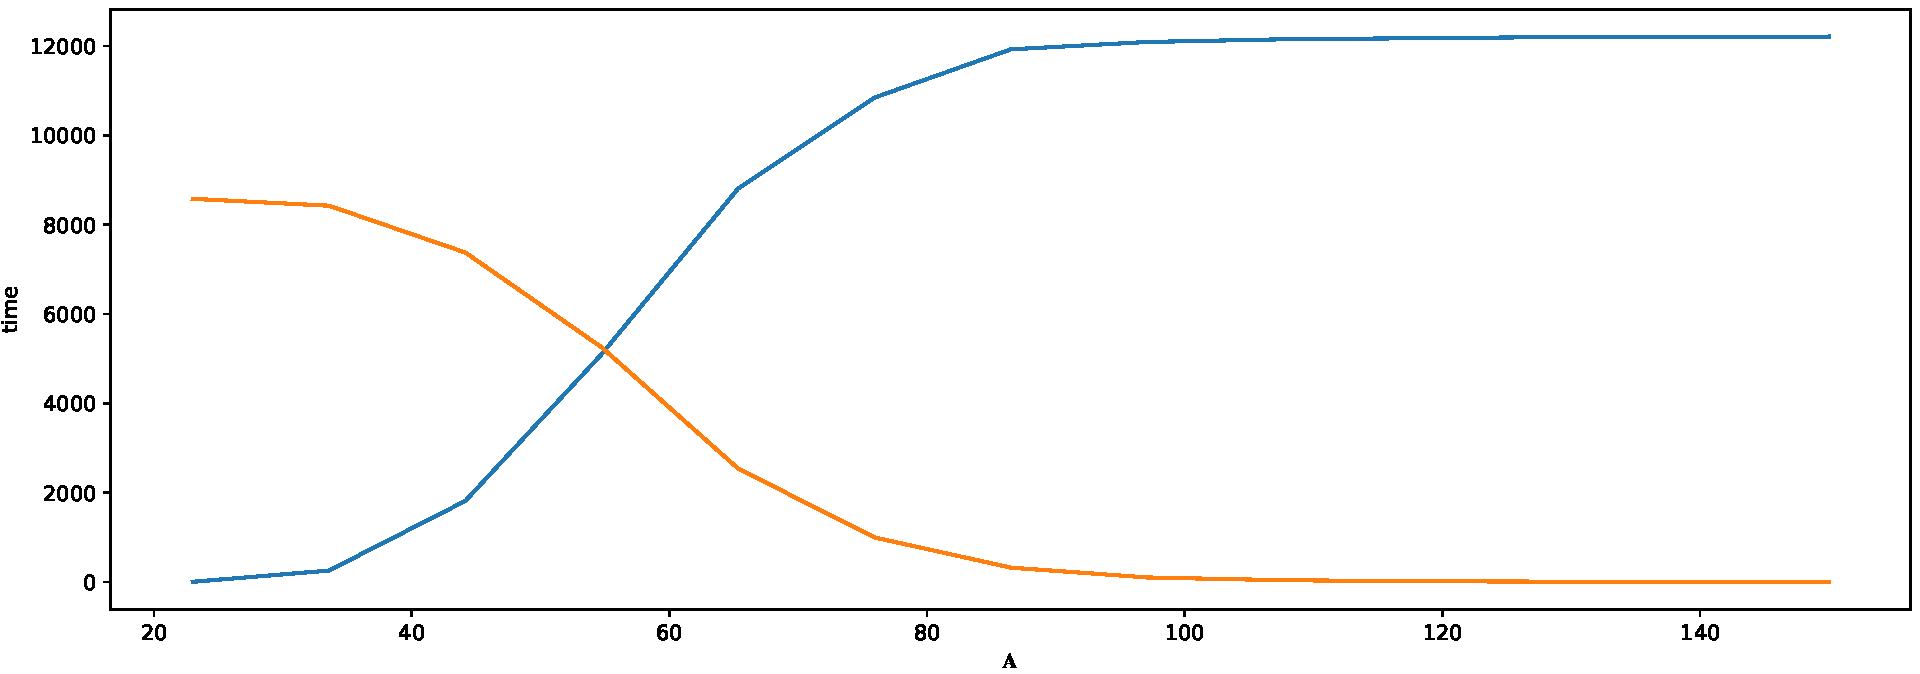
\includegraphics[width=6.0in]{{../Figures/srg_edge_mfpt_simple}.pdf}
\end{center}

The plot can be made much nicer with a bit of configuration:

\begin{center}
    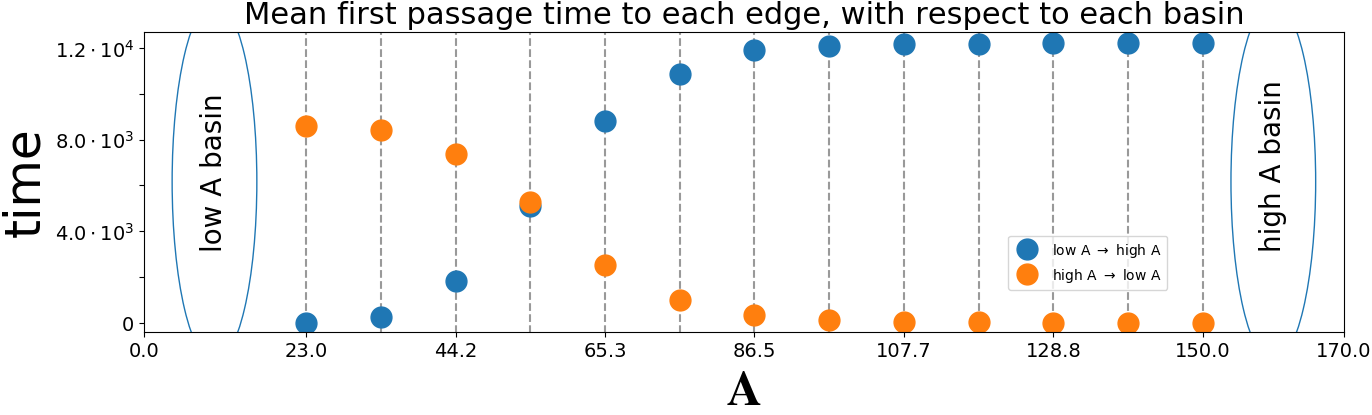
\includegraphics[width=6.0in]{{../Figures/srg_edge_mfpt}.pdf}
\end{center}

the details of which are outside of the scope of this tutorial. However, for the curious, the complete code used to produce the above figure can be found in \pth{\plotterpath}, and a concrete example of its use is in the \pth{\nbpath} notebook.

\subsection{Calculating the MFPT to each tiling edge from the phase weights}

FFPilot simulation calculates the \abr{MFPT} to the $i$th edge of the tiling via a combination of the phase weights, $$\frac{w_0}{\prod_{i=1}^{j} w_i}$$ (as per \eqref{eq:mfpt_from_weights}).
The value of this formula at all of the edges can be quickly calculated using a cumulative product. Given a sequence in which the zeroth term is $w_0$ and remaining terms are the inverse values each $w_{i>0}$, the $i$th element of the cumulative product of this sequence will be the expected value of the time required to reach the $i$th edge:
\begin{equation*}
    \text{cumprod}(\{ w_0, \frac{1}{w_1}, \frac{1}{w_2}, \cdots, \frac{1}{w_N} \}) = \{ w_0, \frac{w_0}{w_1}, \frac{w_0}{w_1 w_2}, \cdots, \frac{w_0}{\prod_{i=1}^N w_i} \}
\end{equation*}

The \code{sfile} package, in conjunction with \code{numpy}, can be used to easily apply this formula:

\inputpy{snippets/srg_mfpt/recalc_mfpt.py}

If you then plot the recalculated \abr{MFPT} values against the \abr{MFPT} values that were originally present in the output file you get:

\begin{center}
    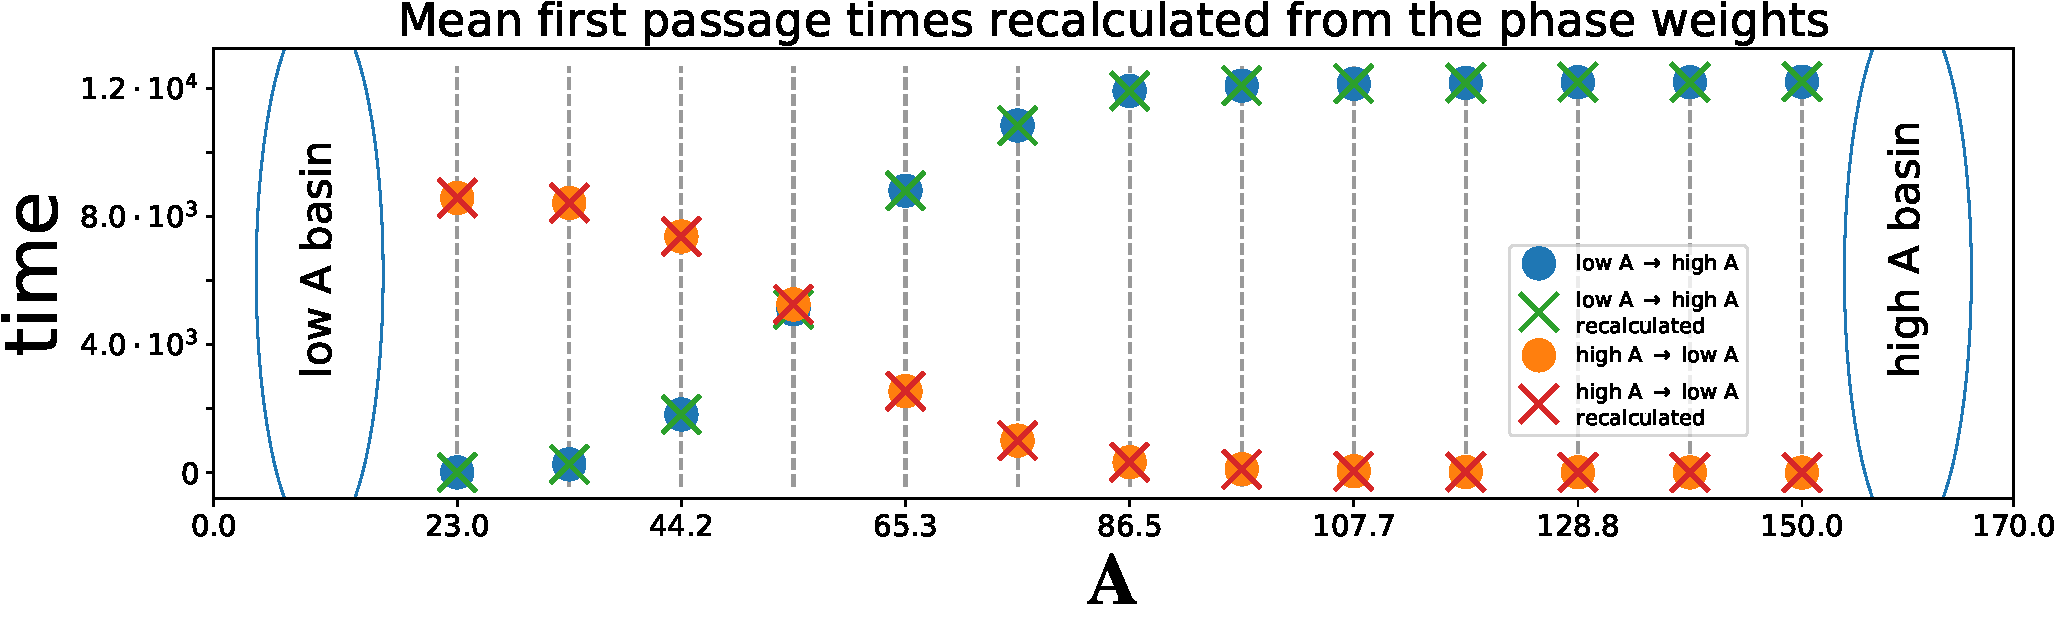
\includegraphics[width=6.0in]{{../Figures/srg_edge_mfpt_recalc}.pdf}
\end{center}

demonstrating that they are indeed identical.

}
\chapter{Calculating the probability landscape of the self regulating gene (SRG) with FFPilot simulation}

\section{Overview}\label{sec:overview_landscape_srg}

Now we move on to the calculation of a system's probability landscape. The landscape is a map which assigns a probability to every occupied state in a system's state space. Producing a landscape from FFPilot output required a much more in-depth post-simulation analysis is needed to get \abr{MFPT} values. However, the simulation itself is very similar.

Just like in chapter 2, we are going to run an FFPilot simulation of the SRG model. In fact, the setup of the simulation input file will be almost identical to that used in the previous chapter. The only difference comes in how the simulation output options are set. A large quantity of data is required to calculate the probability landscape of any given system. When attempting to calculate a highly accurate landscape, the size of the required simulation output files can easily climb into the terrabytes. Thus, landscape output is turned off by default.

Three different types of FFPilot simulation output are required in order to calculate a landscape. Here are the parts of each that are required for the landscape calculation (see \secref{sec:landscape_theory} for full explanations):
\begin{description}[style=nextline]
    \item[SpeciesTimeSeries (turn on with \code{WriteInterval} option)]
        \code{counts} (samples of the species counts)
        \code{first_passage_times} (\abr{MFPT} to each tiling edge)
    \item[FFluxStageOutputRaw (turn on with \code{FFluxStageOutputRaw} option)]
        \code{first_trajectory_ids} (the id of the first trajectory in each phase)\\
        \code{final_trajectory_ids} (the id of the final trajectory in each phase)
    \item[FFluxStageOutputSummary (on by default)]
        \code{weights} (the phase weights)
\end{description}
In brief, binning together the species count samples gives a biased landscape, and the other factors can be used to reweight it into the unbiased landscape.

\section{Set up input for FFPilot landscape simulation of SRG}

In order to create the needed simulation input file, first follow the procedure given in \secrefRange{sec:sbml_conversion_srg}{sec:add_tiling_srg}, but do not follow the instructions for setting the options given in \secref{sec:customize_opts_srg}. Instead, we will set the options needed to get all of the landscape output.

\subsection{Enable landscape output via the FFPilot options}
The following Python script sets all of the options needed for the landscape simulation:

\inputpy{snippets/srg_landscape/add_options.py}

\begin{description}[style=nextline]
    \item[\code{writeInterval}] If set, the species counts of every trajectory will be sampled and written out at the specified interval. For example, if \code{writeInterval} is set to \code{4.0}, samples are taken when the internal time of a trajectory reaches \code{4.0}, \code{8.0}, \code{12.0}, etc.
    \item[\code{ffluxStageOutputRaw}] \code{bool}, defaults to \code{False}. When this flag is set to \code{True}, it turns on output of the "raw" stage record. By default, each stage only saves a "summary" record to the output. The raw record contains a bunch of detailed, lower-level data that is used by FFPilot during a running simulation.  The raw record is needed for certain post-simulation analyses, such as the calculation of the probability landscape.
\end{description}
As in \secref{sec:customize_opts_srg}, \code{errorGoal} is set slightly higher than the default value (\code{.05}) in order to produce a faster (though less accurate) simulation for demonstration purposes.

As a rule of thumb, a good value of \code{writeInterval} is 1 divided smallest rate constant in the model. For the \abr{SRG} model we are using, the smallest rate constant is the one controlling the decay reaction, and it has a value of 1.

\section{Running the simulation}

The simulation is run in an identical fashion to the one we performed in \secref{sec:running_srg_mfpt}:

\inputcmd{snippets/srg_landscape/lmes.sh}

The only noticeable difference should be that the simulation output file is significantly larger than it was before. This is caused by all of the system state samples that get written to the output due to the \code{writeinterval} option being set.

\section{Calculating probability landscapes of SRG from FFPilot output}\label{sec:landscape_srg}

\subsection{Ingesting the phase landscapes from the simulation output}
We begin our analysis of the output of the \abr{SRG} landscape simulation by ingesting the state samples (and other needed data) from the raw simulation output itself. Most importantly, we will bin all of the state samples that were collected during the same phase together into the phase histograms (see \secref{sec:overview_landscape_srg} for details). The following Python script uses the \pth{robertslab.SFile} package to accomplish this:

\inputpy{snippets/srg_landscape/ingest_output.py}

In brief, the script opens the output file and iterates through the records. When it finds a record containing needed data, it performs a particular action based on the record's type:
\begin{description}[style=nextline]
    \item[SpeciesTimeSeries]
        The script retrieves the appropriate phase landscape histogram (one is created for each combination of basin and phase), unpacks the \code{counts} array of the record, and then adds it to that histogram.
    \item[FFluxStageOutputRaw (turn on with \code{FFluxStageOutputRaw} option)]
        The script calculates the count of trajectories run in each phase then stores the results.
    \item[FFluxStageOutputSummary (on by default)]
        The script fetches the \code{weights} and the \code{first_passage_times} and stores them.
\end{description}

The outcome of this script is the creation of a number of python dictionaries that contain all of the data needed for the subsequent analyses. Each of these dictionaries contains exactly two entries, one for each basin/production stage in the simulation we just ran. The nature of these entries is as follow:
\begin{description}[style=nextline]
    \item[\code{basinPhaseHists[i]}]
        The phase hists from the production stage initialized at basin $\ix$.
    \item[\code{basinMFPTs[i]}]
        The \abr{MFPT} to each tiling edge of stage $\ix$.
    \item[\code{basinPhaseWeights[i]}]
        The phase weights of stage $\ix$.
    \item[\code{basinTrajectoryCounts[i]}]
        The total count of trajectories, whether they succeeded or failed, run during each phase of stage $\ix$
\end{description}

\subsection{How histograms are represented in this analysis}

The phase landscape histograms built up by the script will each contain the species count observations collected during a single particular phase. They are represented as Python dictionaries with the following format:
\begin{equation*}
    \begin{array}{cc}
    \text{KEY} & \text{VALUE}\\
    \cdots &\\
    (\speciescountxy{k}{0}, \speciescountxy{k}{1}, \cdots, \speciescountxn{k}) & x_k \\
    (\speciescountxy{k+1}{0}, \speciescountxy{k+1}{1}, \cdots, \speciescountxn{k+1}) & x_{k+1} \\
    \cdots &\\
    \end{array}
\end{equation*}
Where $\speciescountij$ is the $\ix$th observed state (\ie count) of a system's $\jx$ unique chemical species, and $x_\ix$ is the number of times the $\ix$th state has been observed.

For example, from our \abr{SRG} landscape simulation, the contents of the histogram created from the samples collected from phase 4 of the simulation stage initialized from basin 1 may look like this:

\inputpy{snippets/srg_landscape/hist_example.txt}

\subsection{Basic manipulation of histograms}

Before moving on to the landscape calculation proper, we'll first define a few basic functions to help manipulate the histograms:

\inputpy{snippets/srg_landscape/hist_functions.py}
These 4 functions are general histogram operations:
\begin{description}[style=nextline]
    \item[\code{addHists}]
        Adds the values from two histograms \code{h0} and \code{h1} together into a new histogram. For example:
\begin{minted}[escapeinside=||,mathescape=true]{text}
          h0                    h1                addHists(h0,h1)

    [0, 0, 0] |$\rightarrow$| [150]    [0, 0, 0] |$\rightarrow$| [59]      [0, 0, 0] |$\rightarrow$| [209]
    [0, 0, 1] |$\rightarrow$| [141]    [0, 0, 1] |$\rightarrow$| [148]     [0, 0, 1] |$\rightarrow$| [289]
    [0, 1, 0] |$\rightarrow$| [132]    [0, 1, 0] |$\rightarrow$| [152]     [0, 1, 0] |$\rightarrow$| [284]
    [0, 1, 1] |$\rightarrow$| [86]     [0, 1, 1] |$\rightarrow$| [139]     [0, 1, 1] |$\rightarrow$| [225]
    [1, 0, 0] |$\rightarrow$| [90]     [1, 0, 0] |$\rightarrow$| [143]     [1, 0, 0] |$\rightarrow$| [233]
    [1, 0, 1] |$\rightarrow$| [136]    [1, 0, 1] |$\rightarrow$| [154]     [1, 0, 1] |$\rightarrow$| [290]
    [1, 1, 0] |$\rightarrow$| [130]    [1, 1, 0] |$\rightarrow$| [123]     [1, 1, 0] |$\rightarrow$| [253]
    [1, 1, 1] |$\rightarrow$| [135]    [1, 1, 1] |$\rightarrow$| [82]      [1, 1, 1] |$\rightarrow$| [217]
\end{minted}
    \item[\code{calcOParamHist}]
        Takes a histogram of state's (\ie species counts) and converts it to a histogram of order parameter values. Uses the passed-in function \code{oparam} to perform the conversion.
    \item[\code{normHist}]
        Normalizes the values of the histogram. The normalized value $\bar{x}_{\kx}$ associated with the $\kx$th observed state is found with the following simple formula:
        \begin{equation}
            \overline{x_{\kx}} = \frac{x_{\kx}}{\sum_{\kx} x_{\kx}}
        \end{equation}
        where $x_{\kx}$ is the $\kx$th unnormalized observation value. The values of the normalized histogram are gauranteed to sum to 1.0, meaning that a normalized histogram represents a formal probability distribution.
    \item[\code{sparseToDense1D}] Given that \code{h} is a 1D sparse histogram (for example, any histogram returned by \\
    \code{calcOParamHist} when a 1D order parameter is passed in), this function will convert it to a dense histogram. This dense histogram takes the form of two 1D arrays, one for the observations and one for the values.
\end{description}

We will also define a Python version of the 1D order parameter $\oparama$:

\inputpy{snippets/srg_landscape/order_parameter_functions.py}

\begin{description}[style=nextline]
    \item[\code{oparamAlpha}] Takes a species count (as a tuple) for input and returns the value of the order parameter (also as a tuple). For \abr{SRG}, it may seem trivial and unnecessary to store species counts/order parameter values as tuples, since they're always single-valued, or to transform them using a function, since the species count and the order parameter always have the same value. However, writing the code this way makes most of it reusable when we start dealing with systems with higher-dimensional state spaces and order parameters in the next chapter.
\end{description}

\subsection{Calculate the stage histograms}\label{sec:srg_stage_hists}

The first step to calculating the landscape is to take the phase hists from all of the phases that were run during each of the stages and combine them into stage hists. The landscape weights $\landweight$ needed to combine the phases hists within a stage can be calculated from \eqref{eq:landweight} (see \secref{sec:landscape_stage} for details). The following Python script will calculate the $\landweight$ values, weight the phase hists, and then combine them into two stage hists:

\inputpy{snippets/srg_landscape/stage_hists.py}

\begin{center}
    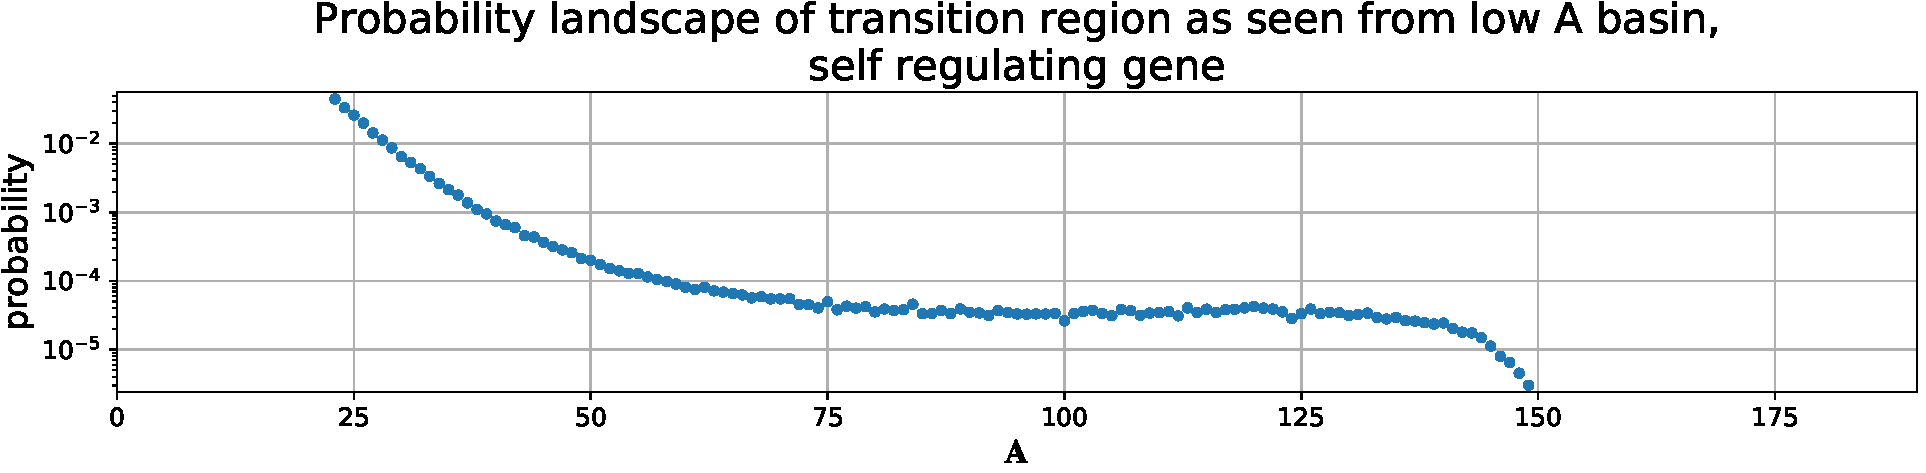
\includegraphics[width=6.0in]{{../Figures/srg_landscape_low_A_basin}.pdf}
\end{center}

\begin{center}
    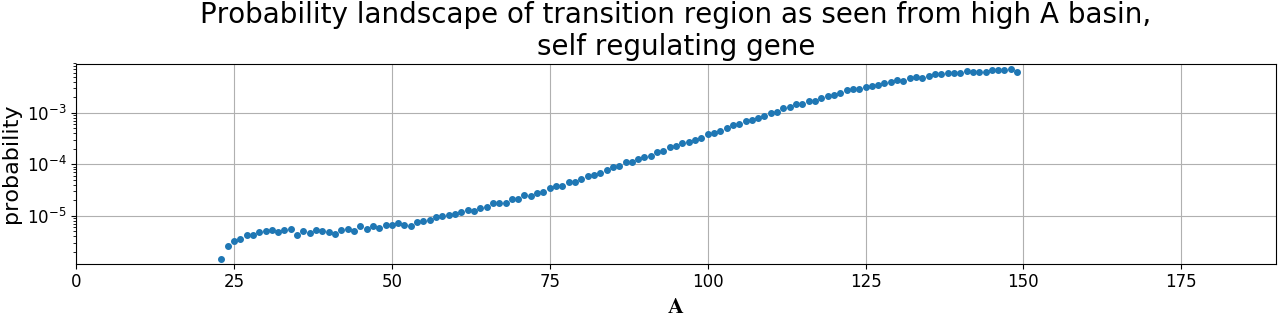
\includegraphics[width=6.0in]{{../Figures/srg_landscape_high_A_basin}.pdf}
\end{center}

\subsection{Combine the stage landscapes into the transition landscape}\label{sec:srg_transition_landscape}
Now we find the transition region landscape by taking the sum of the two stage landscapes weighted by the stage landscape factors $\stageweight$. The following script find the $\stageweight$ values and performs the combination of hists:

\inputpy{snippets/srg_landscape/transition_hist.py}

We now have an unbiased landscape of the \abr{SRG}, though for now it only spans the transition region in between the basins:

\begin{center}
    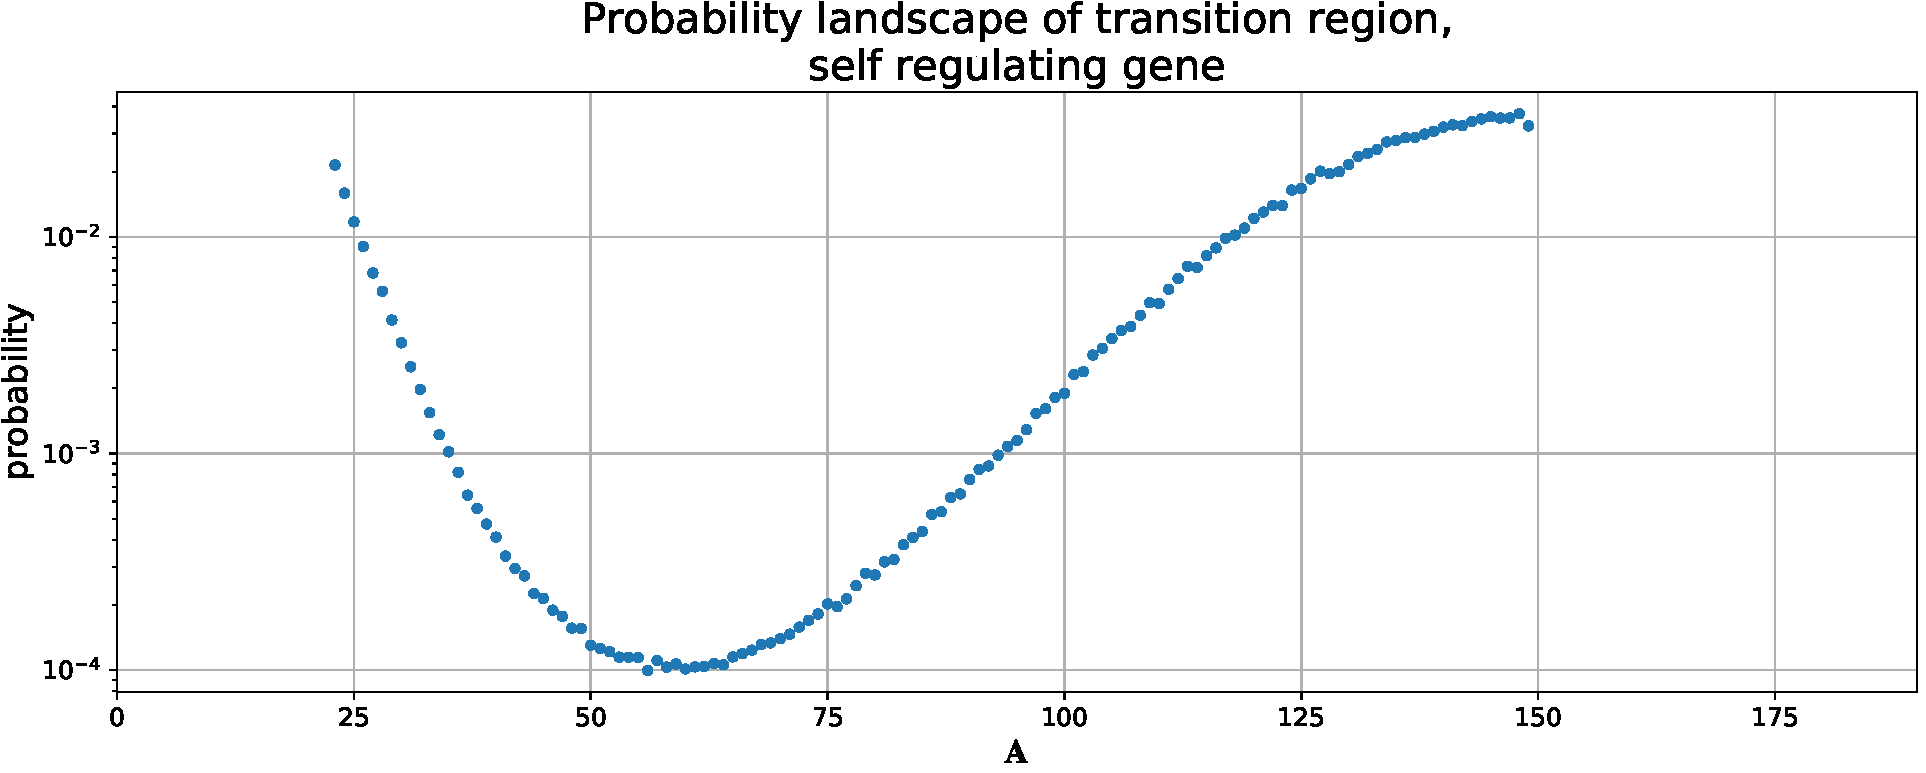
\includegraphics[width=6.0in]{{../Figures/srg_landscape_transition}.pdf}
\end{center}

\subsection{Fit together the complete landscape}\label{sec:srg_complete_landscape}

%As mentioned in \secref{sec:landscape_complete} %(see that section for math-y details)
The final step of assembling the complete landscape is also the most complicated. It proceeds in roughly 3 steps:\\
\\
\textbf{1. Sort all of the phase zero samples into two histograms}\\
One with the samples to the left of the transition minimum, and one with all of the sample to the right. The following script will accomplish this:

\inputpy{snippets/srg_landscape/split_phase_zero.py}

\textbf{2. Fit the left and right phase zero histograms onto the transition region landscape}\\
Independently, we find the weights that will smoothly fit both the left and right phase zero histograms to the transition landscape. We do this using a straightforward minimization approach, with a least-squares minimizer and a Jenson-Shannon divergence\footnote{a symmetrized form of the Kullback-Leibler divergence}. The following script will perform this fitting and report the weights:

\inputpy{snippets/srg_landscape/fit_hists.py}

\textbf{3. Patch together the phase zero histograms and the transition landscape}\\
Finally, we patch the weighted phase zero histograms together with the transition landscape in order to produce the complete landscape. The following script performs this patching:

\inputpy{snippets/srg_landscape/combine_landscape.py}

If any bin in the phase zero histograms overlaps with any bin in the transition landscape, we discard the information from the phase zero histograms in favor of that in the transition landscape, on the assumption that the transition landscape will in general be better sampled.

Now that it's all put together, the complete unbiased landscape looks like this:

\begin{center}
    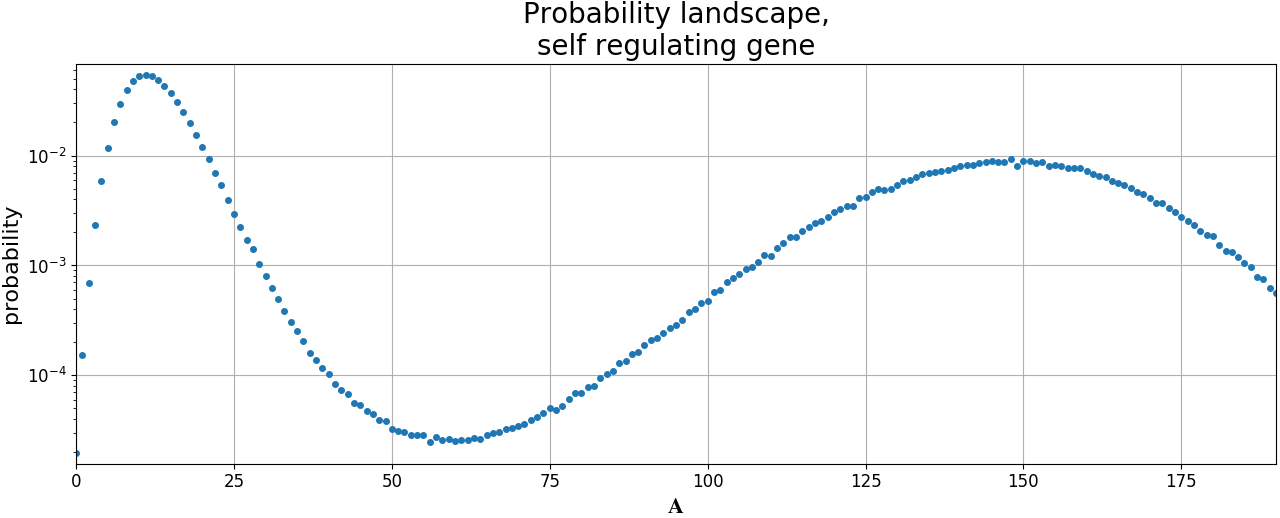
\includegraphics[width=6.0in]{{../Figures/srg_landscape}.pdf}
\end{center}

\subsection{Comparison of landscapes produced using FFPilot and direct sampling}

Shown below are a comparison of landscapes calculated using a (blue dots) 10\% error goal FFPilot simulation and (orange line) direct sampling simulation that collected $10^9$ state samples.

\begin{center}
    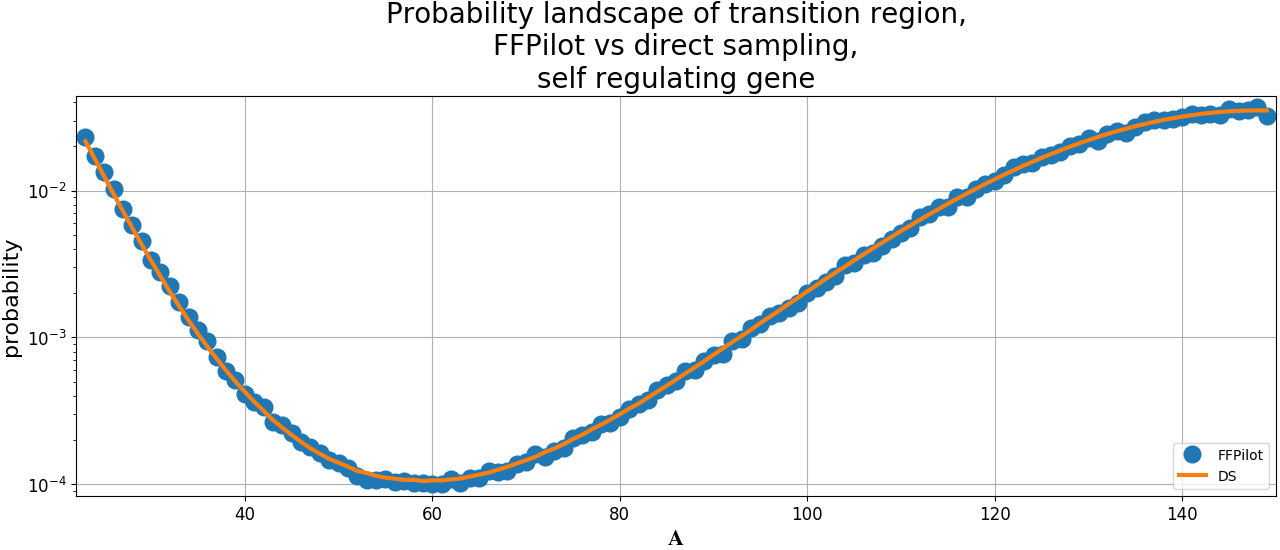
\includegraphics[width=6.0in]{{../Figures/srg_landscape_transition_ffpilot_vs_bf}.pdf}
\end{center}

\begin{center}
    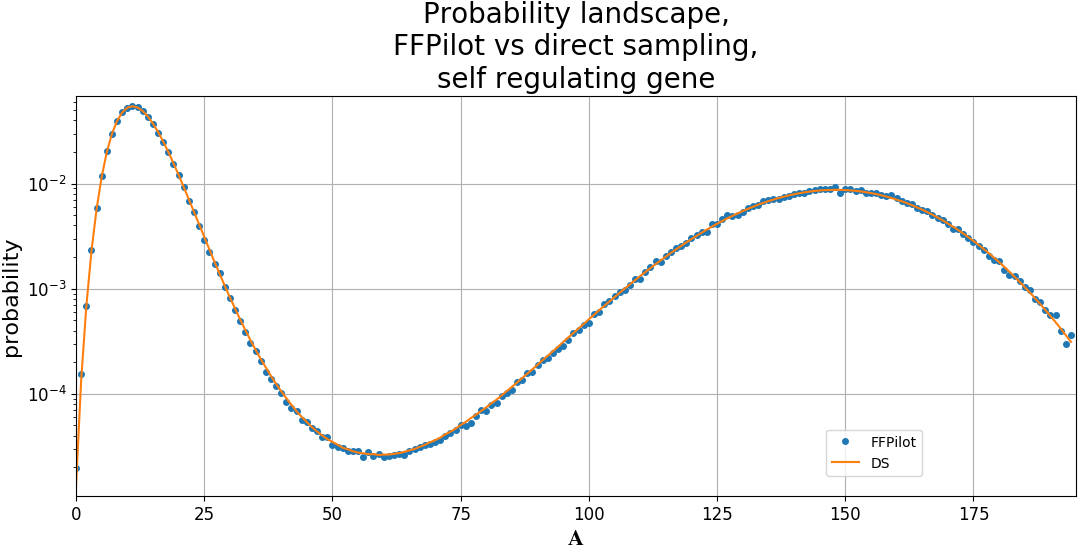
\includegraphics[width=6.0in]{{../Figures/srg_landscape_ffpilot_vs_bf}.pdf}
\end{center}

Although the FFPilot landscape is in this case slightly noisier, overall there is a high level of agreement between the FFPilot and direct sampling landscapes. This is made more impressive by the fact that, in terms of real wall-clock time, the FFPilot simulation ran to completion about 140x faster than the direct sampling one (${\sim}30$ seconds vs ${\sim}70$ minutes).

%\chapter{Tips and tricks for setting up an FFPilot simulation}

\section{Setting up a de novo FFPilot simulation}

There are no hard and fast rules for setting up the order parameter and tiling required for an \abr{FFPilot} simulation. The optimal choice for either of these will be very dependent upon the particular system being simulated. However, it is possible to generate a reasonable order parameter and tiling using a fixed procedure if the coordinates (in terms of a system's state space) of the states of interest are at least roughly known. In other words, although a truly de novo simulation is not possible with FFPilot (or any other forward flux-type method), given a small amount of prior knowledge (in the form of the approximate locations of the system's basins, \ie stable fixed points) it is possible to automatically derive the remaining input required for an FFPilot simulation.

\subsection{Generating a simple linear order parameter}

\subsection{Generating a simple linear tiling}
Each initial basin should either be in front of the zeroth edge or behind the last edge. Mathemtically, this means that one of $$ \mathscr{O}(\text{basin}) < \mathscr{O}(\text{Edges}[0]) $$ or $$ \mathscr{O}(\text{basin}) > \mathscr{O}(\text{Edges}[-1]) $$ should be true, where $\mathscr{O}$ is the order parameter of the tiling.

As a note, FFPilot will automatically recognize when a basin is located behind the last edge of the tiling. In this case, the tiling will be reversed (the last edge will be treated as the zeroth, the zeroth edge will be treated as the last, etc).

\subsection{Caveats}
This order parameter will likely be "naive", in the sense that it will be somewhat computationally inefficient to drive the system along it\footnote{Relative to some optimal order parameter that would drive the system along the true transition pathway.}. However, chances are it will be good enough for use during initial 

\section{Tweaking and tuning an FFPilot simulation}
\subsection{Useful FFPilot simulation options}
{\newcommand{\exampleroot}{\noss{notebooks}}
\newcommand{\gtsname}{\noss{gts}}
\newcommand{\gtsfullname}{\noss{genetic_toggle_switch}}
\newcommand{\gts}{\gtsname}
\newcommand{\dir}{\noss{\exampleroot\bs\gts}}

\newcommand{\data}{data}
\newcommand{\dataw}{\noss{{\data}_worked}}
\newcommand{\sbml}{{\gtsfullname}.sbml}
\newcommand{\lm}{\gtsname.lm}
\newcommand{\out}{\noss{{\gtsname}_out.sfile}}
\newcommand{\lmlog}{\gtsname.log}
\newcommand{\nb}{\gts.ipynb}
\newcommand{\nbw}{\noss{{\gts}_worked.ipynb}}
\newcommand{\plotter}{plotLandscape.py}

\newcommand{\datapath}{\dir\bs\data}
\newcommand{\datawpath}{\dir\bs\dataw}
\newcommand{\sbmlpath}{\exampleroot\bs{\sbml}}
\newcommand{\lmpath}{\datapath\bs\lm}
\newcommand{\outpath}{\datapath\bs\out}
\newcommand{\lmlogpath}{\datapath\bs\lmlog}
\newcommand{\nbpath}{\exampleroot\bs\nb}
\newcommand{\nbwpath}{\exampleroot\bs\nbw}
\newcommand{\plotterpath}{\dir\bs\plotter}

\newcommand{\sbmlpathrel}{..\bs\sbml}
\newcommand{\lmpathrel}{\data\bs\lm}
\newcommand{\outpathrel}{\data\bs\out}
\newcommand{\lmlogpathrel}{\data\bs\lmlog}

\chapter{Using FFPilot to simulate systems with complex, high-dimensional state spaces: genetic toggle switch}

\section{Overview}

In this chapter, we'll be working with the genetic toggle switch (GTS). \abr{GTS} is to the study of genetic regulatory systems what the hydrogen atom was to the study of quantum mechanics. It is one of the simplest truly biphasic systems that has actually been experimentally instantiated in living cells\cite{Gardner:2000bm}. \abr{GTS} models come in many different variants, and we will work with one called the exclusive genetic toggle swtich. It consists of 7 distinct chemical species that participate in 14 separate reactions.

\begin{center}
    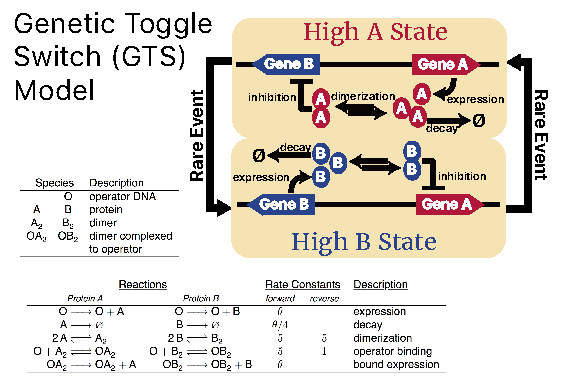
\includegraphics[width=6in]{{../Figures/model_schematics/genetic_toggle_switch}.pdf}
\end{center}

Protein A and protein B are both produced from a single piece of operator DNA. A and B can both dimerize, and each dimer can bind back to the operator DNA. Only one dimer can bind to the DNA at a time. When the DNA is unbound, it will produce both A and B at an equal rate. However, when a dimer of one of the proteins is bound, the DNA will only produce more of that same protein. This means that \abr{GTS} spends the vast majority of its time in either a high A, low B state (state $\statea$), or a high B, low A state (state $\stateb$).

\abr{SRG} has 1 unique chemical species, and thus a 1D state space. \abr{GTS} has 7 unique species and a 7D state space, and so is inherently a much more complex system to simulate and analyze. In particular, complex sources of error emerge in higher dimensional systems that aren't present in 1D systems like \abr{SRG}. Helpfully, \abr{GTS} has a feature that makes it easy to examine simulation error: it's perfectly symmetric in terms of proteins A and B. In fact, because the species and reactions containing A are identical to those containing B (aside from, of course, the change in protein), the \abr{MFPT} of the $\atob$ transition is equal to that of $\btoa$, and the probability landscape of \abr{GTS} is perfectly symmetrical. The deviation from this 2-fold symmetry can thus be used as a simple measure of simulation accuracy.

Over the course of the previous chapters in this tutorial we established the theory and protocols for running and analyzing FFPilot simulations. In this chapter we'll focus on error, and how to think about simulation accuracy in general.

\section{FFPilot simulation input for GTS}

The protocol for setting up the input for an FFPilot simulation of \abr{GTS} is very similar that used in the earlier chapters for setting up simulations of \abr{SRG}. Essentially, certain array values, such as \code{\oparamcoeffs} and \code{\tilingbasins}, which were 1D for \abr{SRG} are 7D for \abr{GTS}. Although this may sound complex, in practice it is not much more complex than setting up \abr{SRG}.

Once again, we're going to use the \exe{lm_sbml_import} to convert a \path{.sbml} file to an \path{.lm} file, and then use the \code{h5py} Python package to add the needed order parameter and tiling.

First, we run the \exe{lm_sbml_import} utility on \pth{\sbml} in order to produce \pth{\lm}. Open a terminal, then \sh{cd} to \pth{\dir} and then execute:

\inputcmd{snippets/gts/lm_sbml_import.sh}

Next we set the order parameter, the tiling, and the FFPilot simulation options needed for landscape output using the following Python scripts:\\
\\
\textbf{order parameter}

\inputpy{snippets/gts/add_order_parameter.py}

\textbf{tiling}

\inputpy{snippets/gts/add_tiling.py}

\textbf{FFPilot simulation options}

\inputpy{snippets/gts/add_options.py}

\section{Running the simulation}
No surprises here, as the \abr{GTS} simulation can be executed with the same basic command that was used to run the \abr{SRG} simulations:

\inputcmd{snippets/gts/lmes.sh}

\section{MFPT to each edge of GTS tiling}

As with our \abr{SRG} simulations, the \abr{MFPT} values of \abr{GTS} can be fetched directly from the simulation stage summary records. Follow the instructions given in \secref{sec:fetch_mfpt_srg} in order to retrieve the \abr{MFPT} results from the \abr{GTS} simulation we just ran. Plotting those values should yield something along the lines of:
 
\begin{center}
    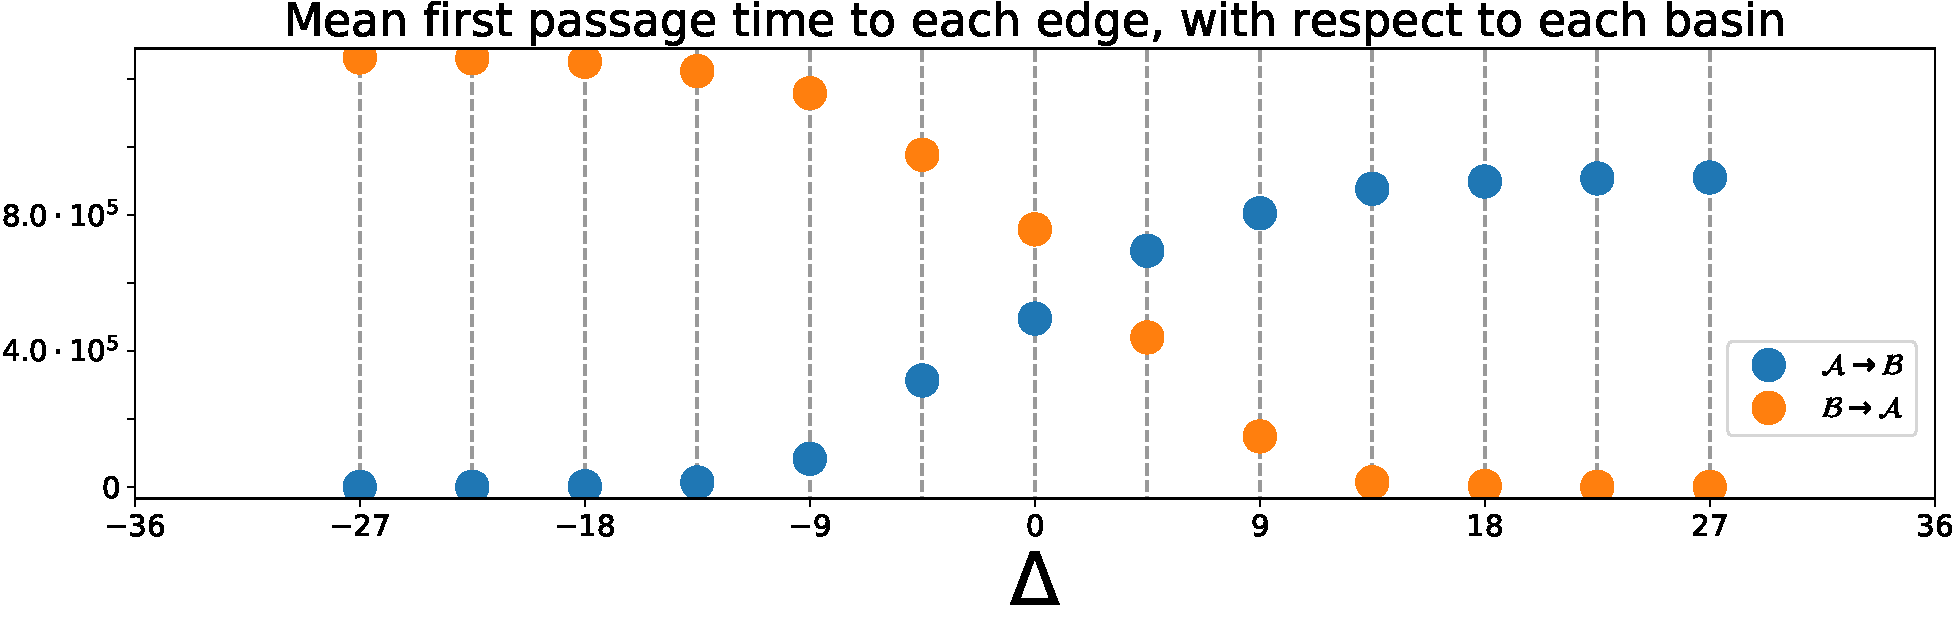
\includegraphics[width=6.0in]{{../Figures/gts_edge_mfpt}.pdf}
\end{center}

There are two sets of GTS MFPT values, those collected when switching $\atob$ and when switching $\btoa$. Regardless of what kind of simulation was used to estimate them, they should be perfectly symmetrical. This means that if one set is flipped with respect to its edges, the two sets would then be equal. However, complete equality is unlikely to be observed in the results from a 10\% error goal simulation. Instead, it is far more likely that some deviation between the two sets of MFPTs will occur:

\begin{center}
    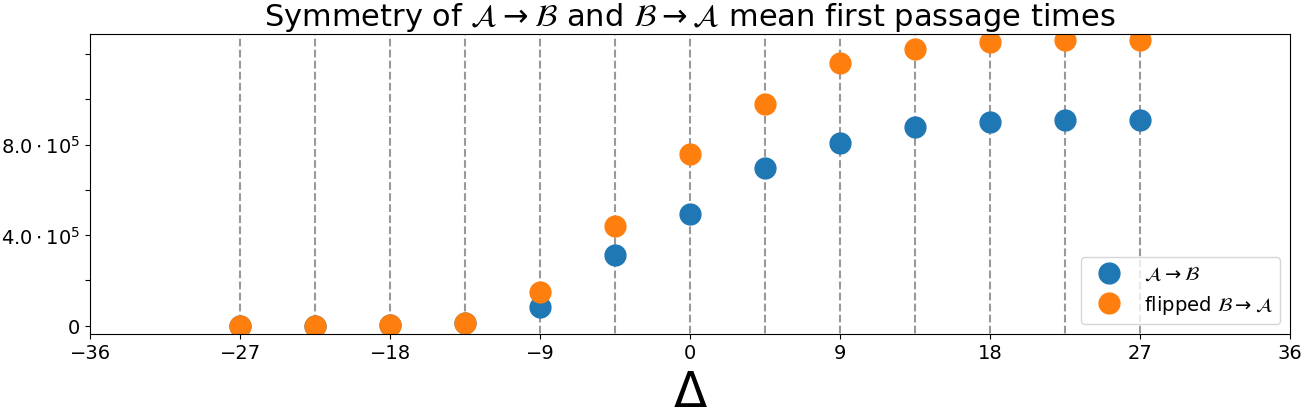
\includegraphics[width=6.0in]{{../Figures/gts_edge_mfpt_symmetry}.pdf}
\end{center}

When GTS is simulated using a 1\% error goal, much less deviation occurs between the results from the $\atob$ and $\btoa$ processes:

\begin{center}
    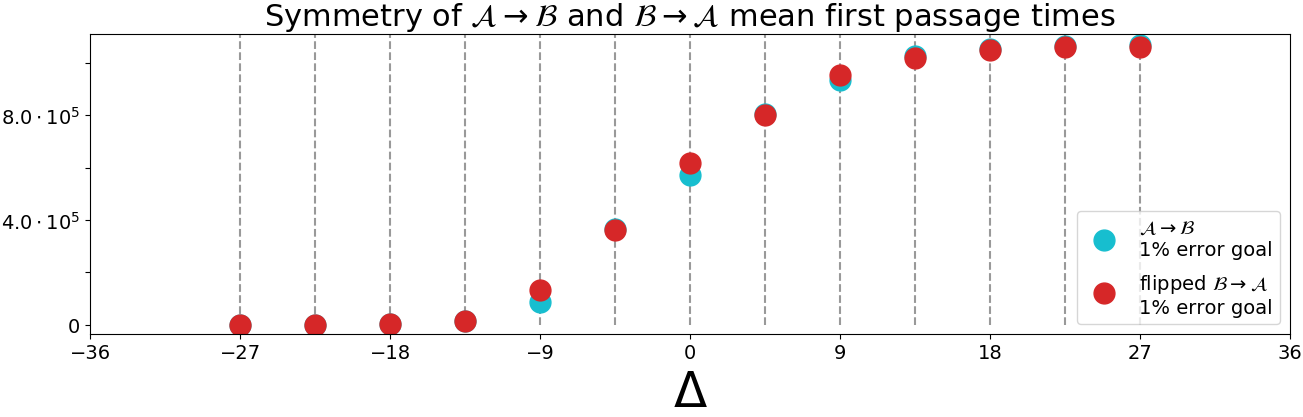
\includegraphics[width=6.0in]{{../Figures/gts_edge_mfpt_symmetry_err_01}.pdf}
\end{center}

As can be seen above, even though some deviations do begin to develop in phases immediately before or around the transition midpoint (\ie $\Delta = 0$), the simulation recovers from those deviations, and they do not persist into the overall basin-to-basin \abr{MFPT} estimates. This can be though of as a signature of the technique which FFPilot uses to optimize computational efficiency. The optimizing equation that drives FFPilot tends to bias simulations against running too many trajectories during the most expensive phases (for \abr{GTS}, the most expensive phases are indeed those in the vicinity of the transition midpoint), and makes up for any errors this might introduce by causing more simulations to be run during the least expensive phases.

\section{Landscape of the transition region}
The code we introduced last chapter in \secref{sec:landscape_srg} for calculating the landscape of \abr{SRG} is flexible enough to be reused almost in its entirety when calculating the landscape of the very different \abr{GTS}. The only major differences are that we will use the \abr{GTS} specific 1D order parameter $\oparamd$, and also define a 2D order parameter $\oparamab$ to do some fancy plotting with:

\inputpy{snippets/gts/order_parameter_functions.py}

\subsection{Calculating the transition region landscape}

The code from \secref{sec:srg_stage_hists} can be used to produce the \abr{GTS} stage histograms:

\begin{center}
    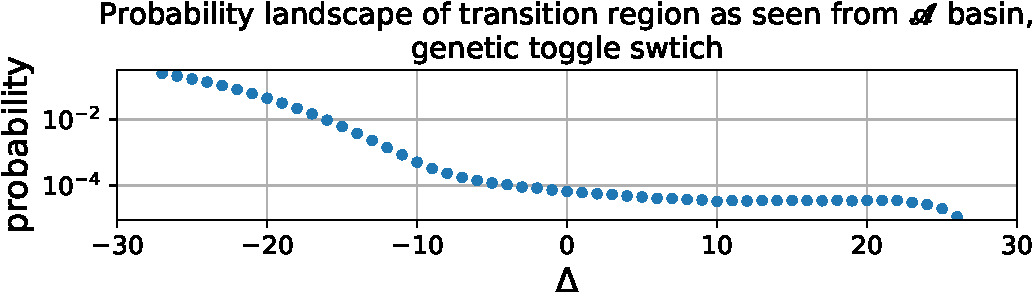
\includegraphics[width=6.0in]{{../Figures/gts_landscape_0_basin}.pdf}
\end{center}
\begin{center}
    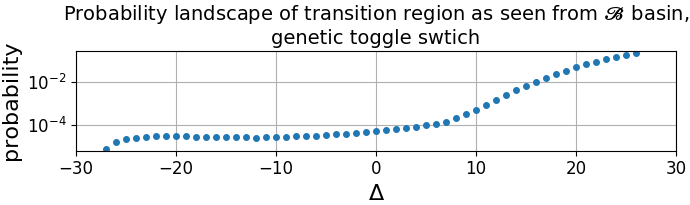
\includegraphics[width=6.0in]{{../Figures/gts_landscape_1_basin}.pdf}
\end{center}

The \abr{GTS} stage histograms can then be combined into a single transition region landscape using the code from \secref{sec:srg_transition_landscape}:

\begin{center}
    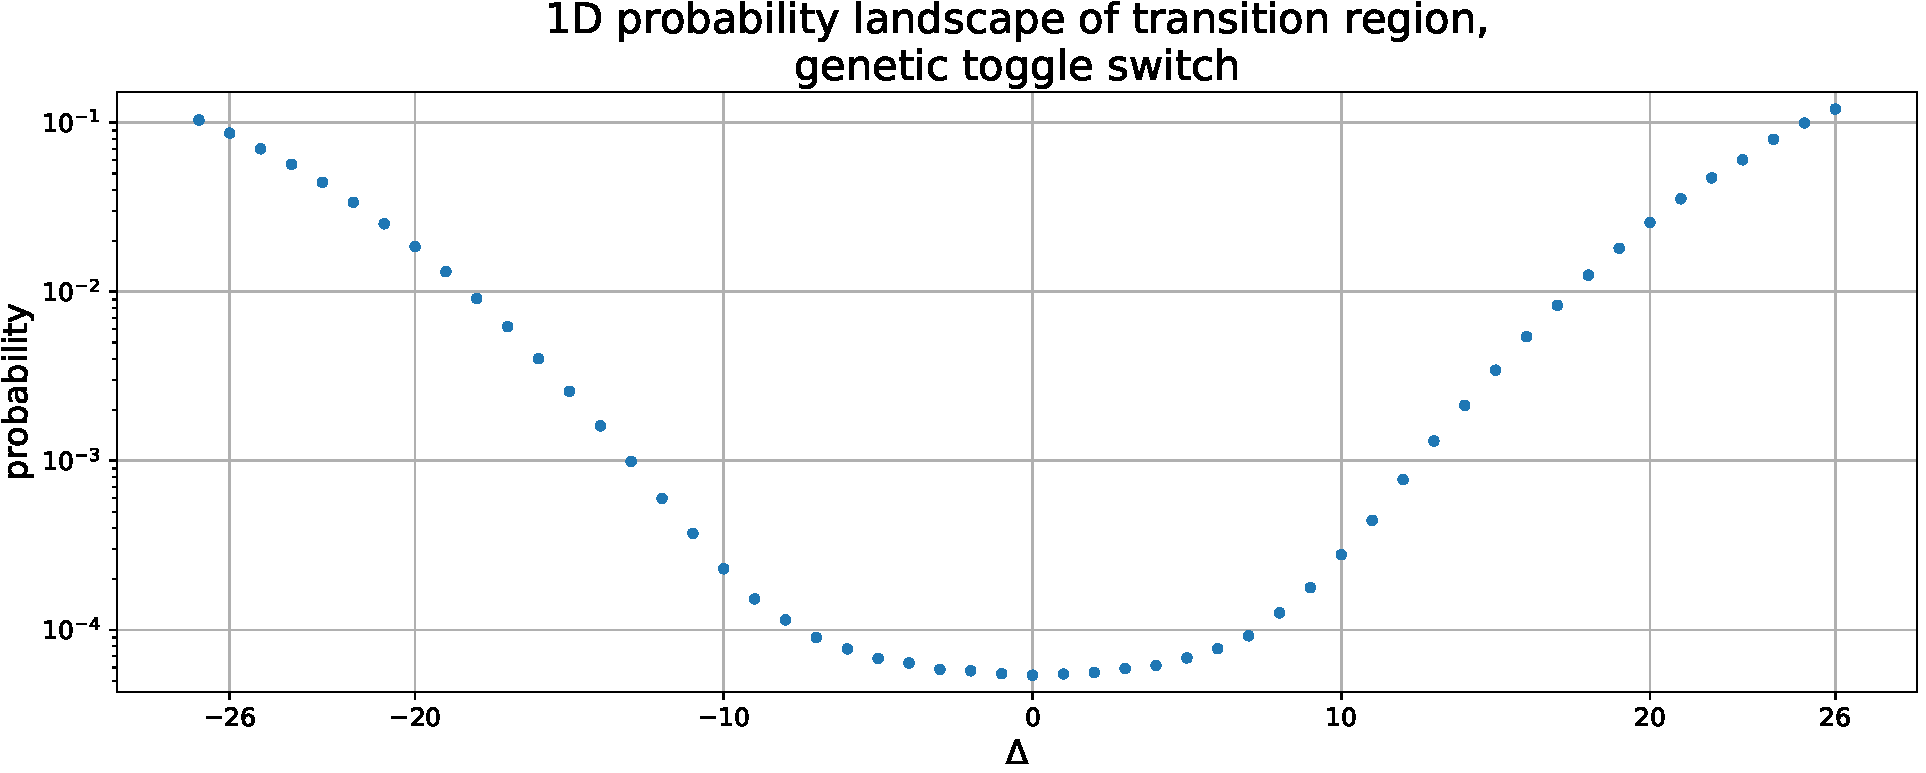
\includegraphics[width=6.0in]{{../Figures/gts_landscape_transition_1d}.pdf}
\end{center}

A great deal more detail can be gleaned when the transition is plotted using the 2D $\oparamab$ order parameter:

\begin{center}
    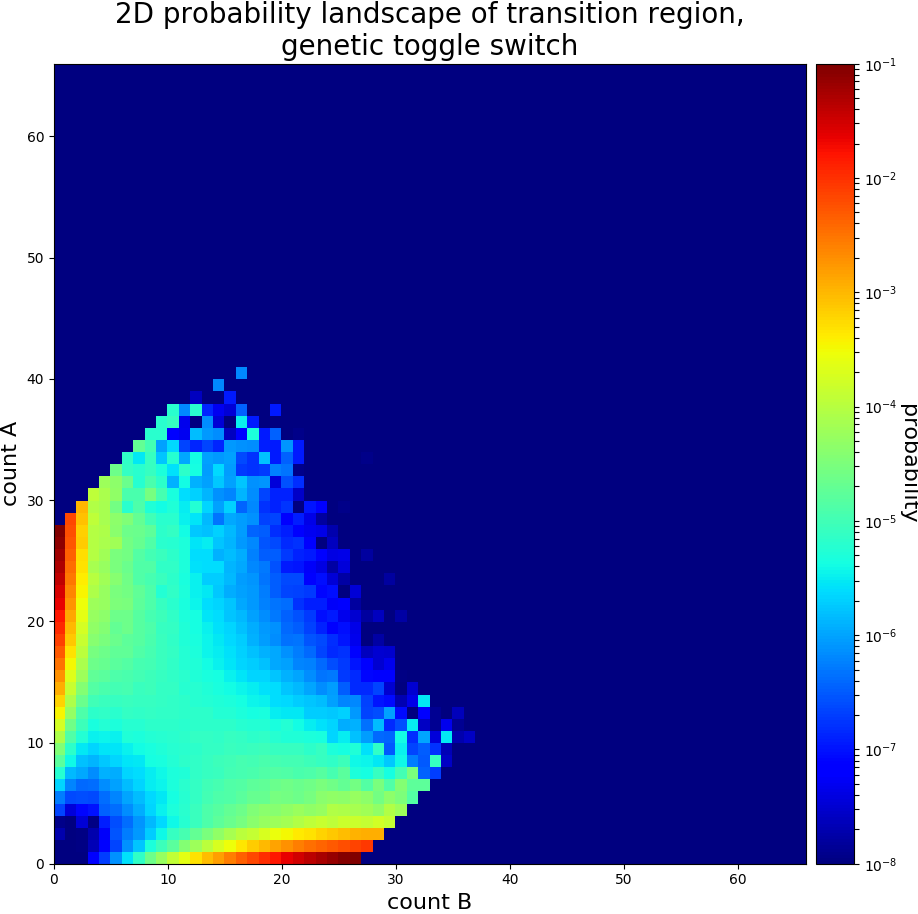
\includegraphics[width=6.0in]{{../Figures/gts_landscape_transition_2d}.pdf}
\end{center}

\subsection{Accuracy of the calculated transition region landscape}

In terms of the 1D order parameter $\Delta$ (ie $\text{count A} - \text{count B}$), the GTS landscape is symmetric over the origin. In terms of the 2D order parameter $\{\text{count A}, \text{count B}\}$, GTS is symmetric over the line $x=y$. These symmetries are important, since they offer a simple way to test the accuracy of our landscape assembly procedure (which includes both the simulation and the analysis). For any landscape we calculate, the closer its two halves are to perfect symmetry the more accurate the assembly procedure was.

Symmetry, or lack thereof, is usually easier to spot in plots of 1D order parameters. Though somewhat analytically crude, a comparison of any two symmetric points ${-x, x}$ in the landscape can be used as a simple, quantitative measure of the landscape's overall accuracy. A sense of how FFPilot error goal affects the accuracy of the landscape can be gained by comparing the two symmetric points $\Delta=-26$ and $\Delta=26$. When a landscape is calculated from a 10\% error goal FFPilot simulation, the divergence between the probabilities of -26 and 26 tends to be quite large, on the order of $10-20\%$:

\begin{center}
    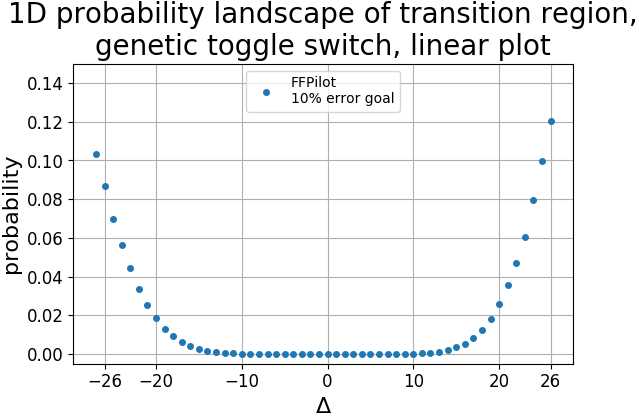
\includegraphics[width=6.0in]{{../Figures/gts_landscape_transition_1d_linear}.pdf}
\end{center}

 On the other hand, as in the plot shown below, the probabilities of -26 and 26 are nearly equal when calculated using data from a 1\% error goal simulation:

\begin{center}
    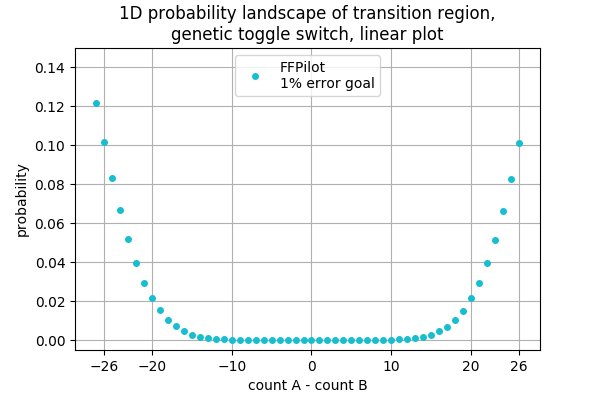
\includegraphics[width=6.0in]{{../Figures/gts_transition_1d_err_01}.pdf}
\end{center}

The landscape shown above was produced from the example data included with the notebook (in the \pth{example_arrays/landscape_ffpilot_basin_\%d.npz} files).

\section{The complete unbiased landscape of GTS}

\subsection{Calculating the complete landscape}
Now that we have the transition landscape assembled, the complete landscape can be calculated by simply reusing the code from \secref{sec:srg_complete_landscape}. Plotted in 1D (along the $\oparamd$ order parameter) and 2D (along the $\oparamab$ order parameter) it looks like:

\begin{center}
    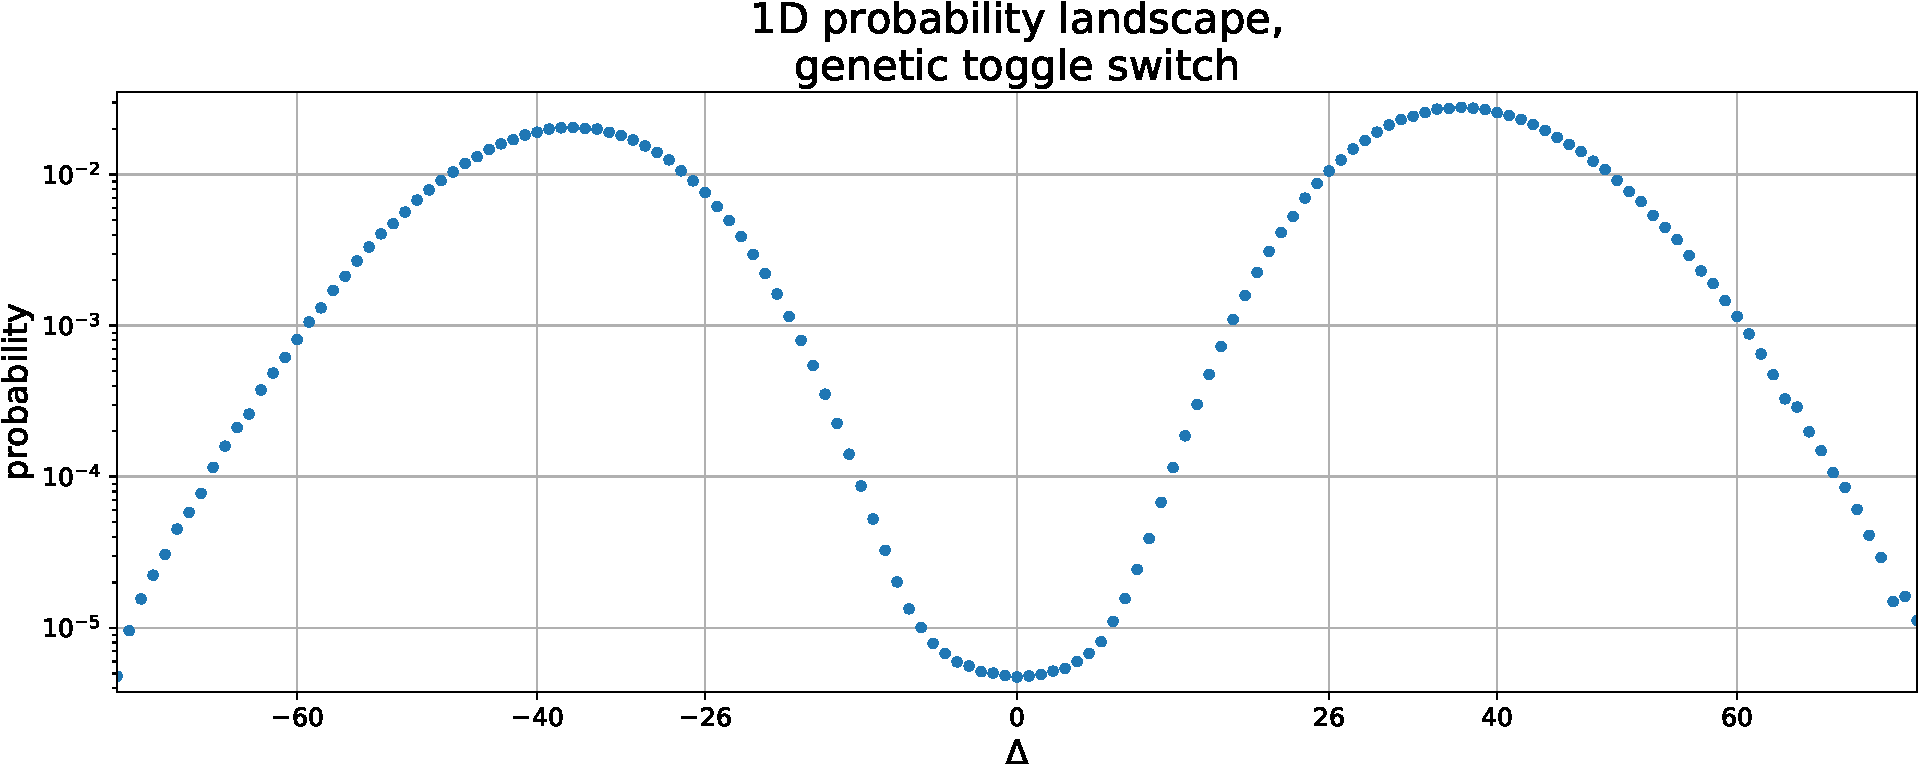
\includegraphics[width=6.0in]{{../Figures/gts_landscape_1d}.pdf}
\end{center}

\begin{center}
    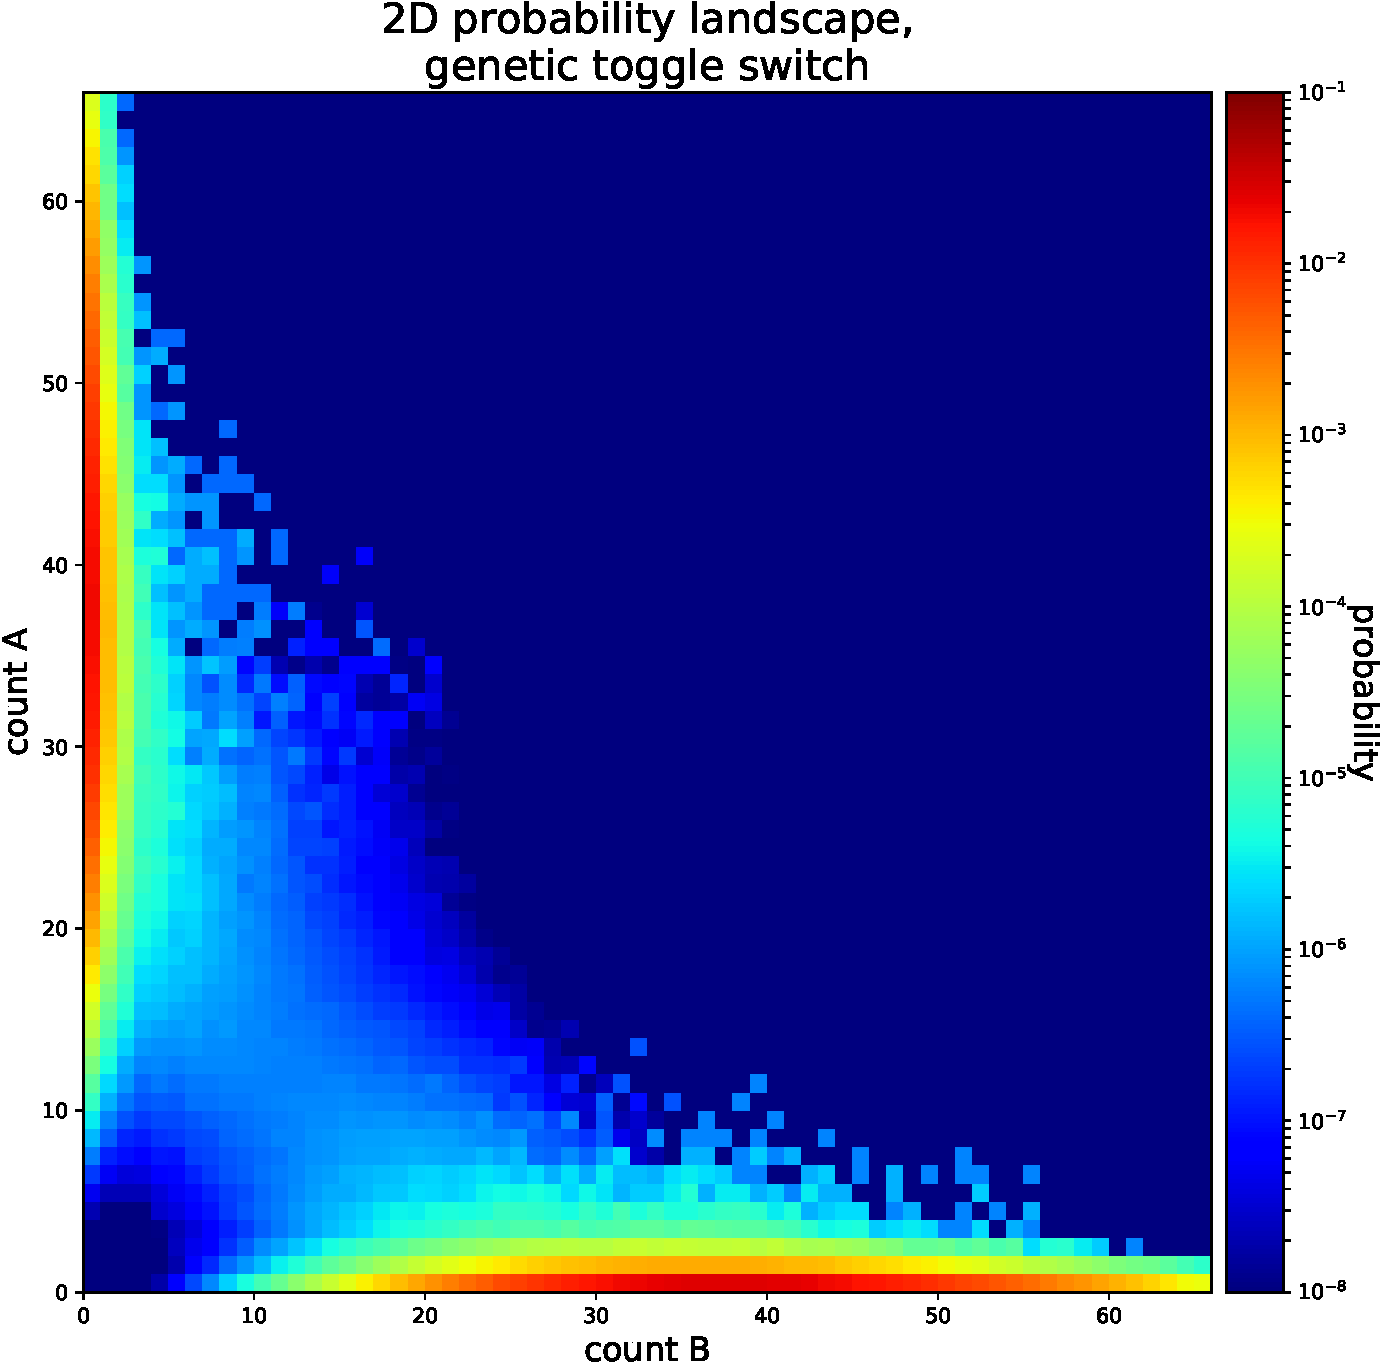
\includegraphics[width=6.0in]{{../Figures/gts_landscape_2d}.pdf}
\end{center}

As you can see above, the fitting procedure in the code we wrote last chapter is robust and flexible enough that it is able to deal with both the \abr{SRG} and the (very much different) \abr{GTS} models.

\subsection{Accuracy of calculated complete landscape: comparison with replicate sampling}
In addition to comparing them against each other, we can also gauge the accuracy of the  two halves of a \abr{GTS} FFPilot simulation by comparing them to the results from a \abr{DS} simulation. Though \abr{DS} simulation is computationally inefficient, it is highly accurate. It has been shown\cite{Gillespie:2007bx} that \abr{DS} simulation will converge roughly monotonically to the correct answer under a large variety of conditions. This convergence behavior, along with a history of decades of use and verification, allows \abr{DS} results to be used as a sort of gold standard when examining novel simulation methods. Here is a comparison of the transition region calculated by FFPilot and \abr{DS} simulations:

\begin{center}
    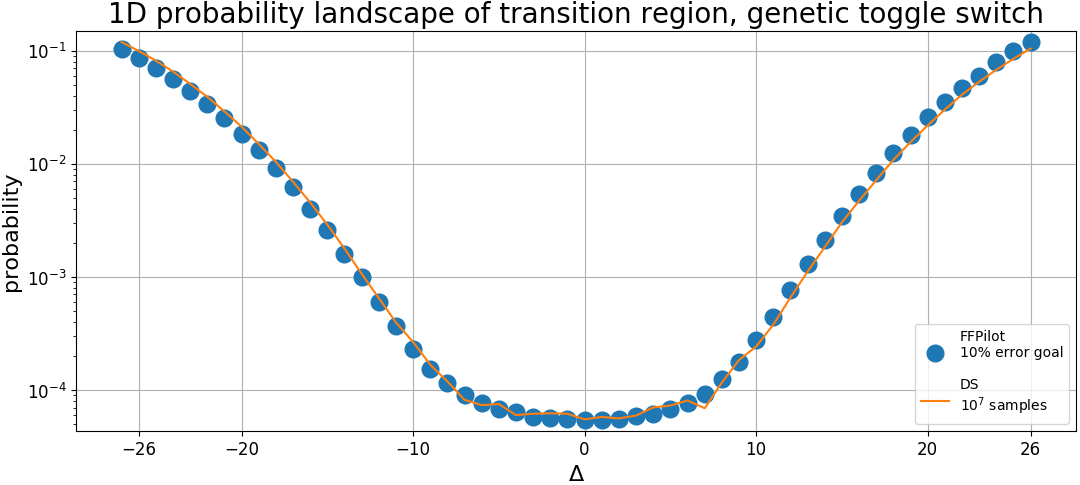
\includegraphics[width=6.0in]{{../Figures/gts_landscape_transition_vs_bf}.pdf}
\end{center}

The landscape produced by FFPilot is much less noisy than the landscape from direct sampling in the immediate neighborhood of the transition point. In terms of landscapes, FFPilot simulation is at its most useful in any region of extremely low probability. Direct sampling tends to struggle with these low probability regions, and can only collect enough samples to map their landscapes with reasonable accuracy when vast computational resources are used.

This version of the genetic toggle switch is completely symmetric in terms of A and B. Thus, the two peaks in the probability distribution should be the same height. The peak on the left corresponds to state $\mathcal{A}$ (in which there is a high count of protein A and a low count of protein B) and the peek on the right corresponds to state $\mathcal{B}$ (in which there is a high count of protein B and a low count of protein A). In terms of the 1D $\oparamd$, the two peeks $\mathcal{A}$ and $\mathcal{B}$ fall at -37 and 37, respectively.

\begin{center}
    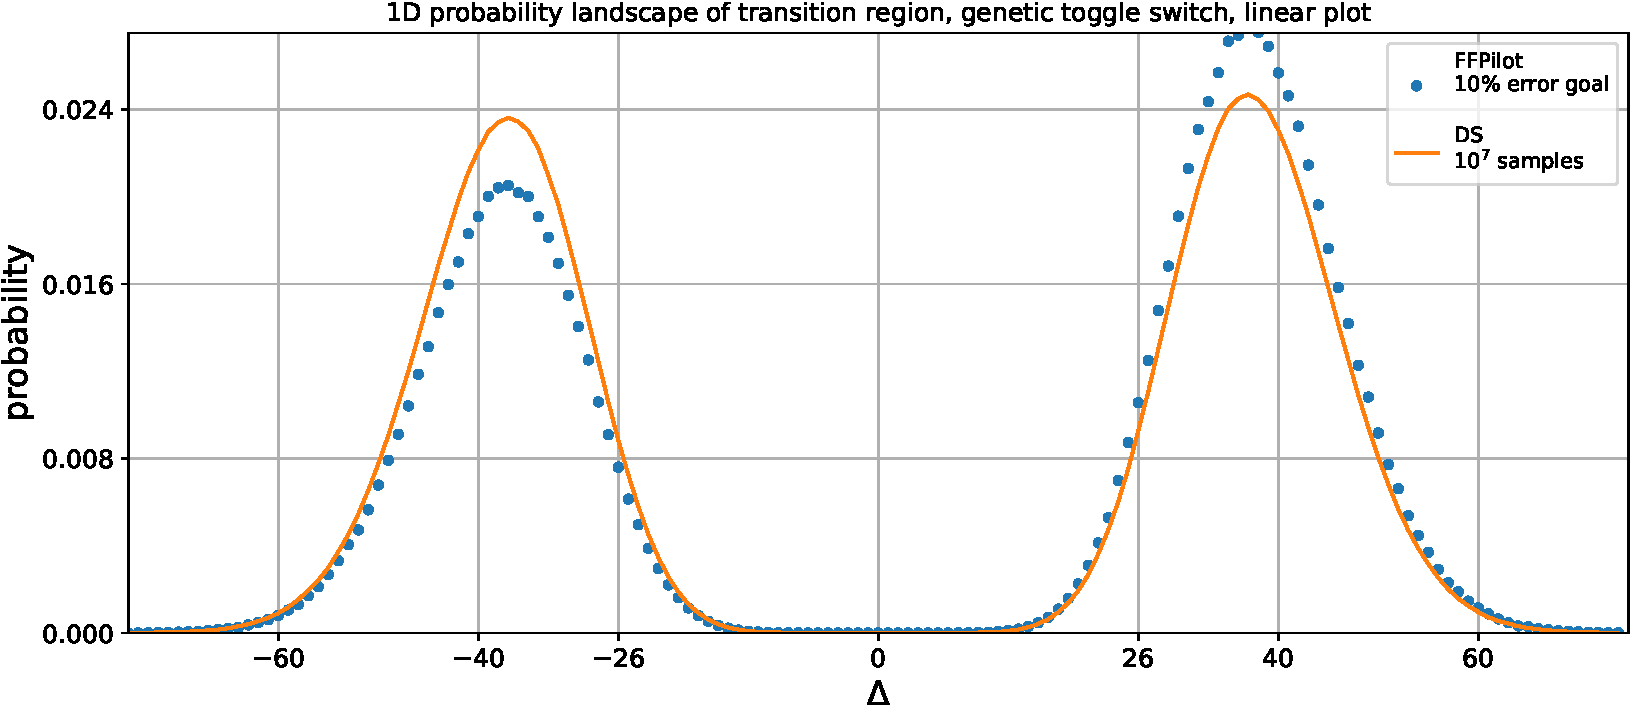
\includegraphics[width=6.0in]{{../Figures/gts_landscape_vs_bf_linear}.pdf}
\end{center}

In the direct sampling data we show above, the height of the state $\mathcal{A}$ and state $\mathcal{B}$ peeks differ by about ${\sim}4.5\%$ relative to one another. Whether FFPilot under- or out-performs this figure depends on the error goal with which a simulation is run. Error goal is expressed in terms of a desired level of error in the estimated MFPT from a simulation, but a lower error goal also tends to reduce error in other measures as well, including this landscape symmetry measure.

In landscapes produced from FFPilot simulations run at an error goal of 10\%, the two peeks can differ by 10\% or more. However, the difference in the peeks decreases dramatically for FFPilot simulations run with a 1\% error goal. The landscape shown below was produced from the example data included with the notebook (in the \\
\code{data_example/landscape_ffpilot_basin_\%d.npz} files), which was obtained from an FFPilot simulation run with a 1\% error goal:

\begin{center}
    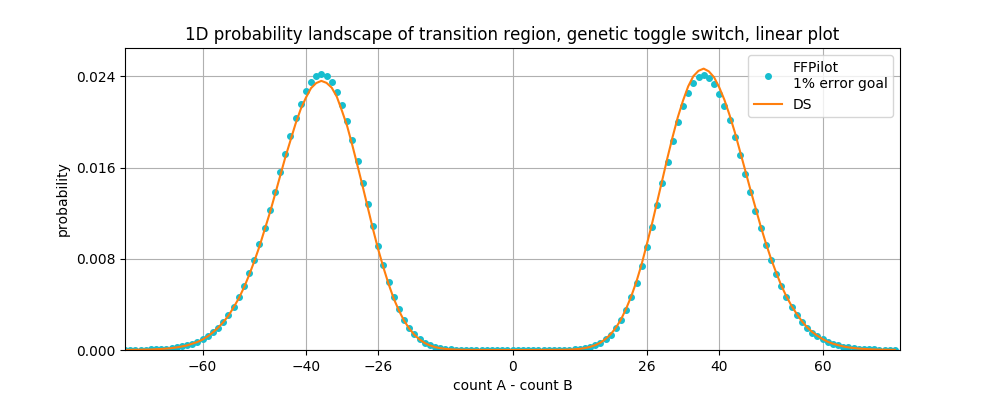
\includegraphics[width=6.0in]{{../Figures/gts_land_1d_err_01_linear}.pdf}
\end{center}

In the landscape produced by FFPilot the heights of the $\mathcal{A}$ and $\mathcal{B}$ peeks are closely matched, and differ by less than 0.7\%. In this case FFPilot outperformed direct sampling in terms of correctly reproducing the underlying symmetry of the genetic toggle switch's landscape.
}


% appendices
\newpage
\appendix
\setcounter{chapter}{0}
\chapter{Setting up FFPilot simulation input using the HDFView gui}

\section{Overview}

\section{Self regulating gene setup}
\begin{enumerate}
    \item Convert the \file{self_regulating_gene.sbml} file to the standard \file{.lm} simulation input format, following the instructions given in \todo{ref to converting from sbml in lmesgs}.
    \item Use \file{HDFView} to manually add the FFPilot-specific simulation input to the resulting \\ \file{self_regulating_gene.lm} file:
    \begin{enumerate}
        \item Open \file{self_regulating_gene.lm} in \file{HDFView}. \file{HDFView} is the standard file browser for \file{.hdf5} files and is available on the \href{HDF Group's website}{https://support.hdfgroup.org/products/java/hdfview/}.
        \item{Add the order parameter:}
        \begin{enumerate}
            \item\label{item:add_group} Right click on \file{self_regulating_gene.lm} in the column on the left, and then select \gui{New $\rightarrow$ Group}. Enter \code{OrderParameters} as the new group's name and then hit \gui{Ok}.
            \item Right click on the new \code{OrderParameters} group and then repeat \ref{item:add_group} in order to create a new subgroup named \code{0000000}. NB: make sure the subgroup name is exactly seven zeros (internally, \code{LMES} uses a seven digit fixed-width format (c-style format \code{\%07d}) for this subgroup name). \todo{If it's quick, refactor the LMES hdf5 stuff to remove the fixed width requirement for input}.
            \item Right click on \code{0000000}, choose \gui{Show Properties}, and then click on the \gui{Attributes} tab in the properties window. Add two attributes, \code{ID} and \code{Type}. Both should be 64-bit integer scalars, and both should have a value of 0.
            \item Add a dataset called \code{SpeciesCoefficients} to the \code{0000000} group. It should be of type 64-bit float, and it should have a size of 1. Double click on \code{SpeciesCoefficients} to open it, and then set its single value to \code{1.0}.
            \item Add another dataset to \code{0000000}. Name this one \code{SpeciesIDs}, set its type to 32-bit unsigned integer, and set its size to 1. Open \code{SpeciesIDs} and make sure that its single value is set to 0 (which it should be by default).
        \end{enumerate}
        \item{Add the tiling (also called the interfaces, or the bins):}
        \begin{enumerate}
            \item Add a \code{Tilings} group with a \code{0000000} subgroup, just as you did for \code{OrderParameters}.
            \item Set three attributes on the \code{0000000} subgroup, \code{ID}, \code{OrderParameterID}, and \code{type}. All of them should be 64-bit integer scalars with a value of 0.
            \item Add a dataset called \code{Basins} to \code{0000000}. It should be of size 1, of type 32-bit unsigned integer, and its single value should be set to 10.
            \item Add a dataset called \code{Edges} to \code{0000000}. \code{Edges} should be of type 64-bit float, and should have a size of 13. The first value should be \code{23.0}, the last value should be \code{150.0}, and the remaining values should be evenly spaced in between. The easiest way to enter these values is to import them from \\ \file{files/self_regulating_gene_mfpt/edges.txt}, a plain text file that contains the needed values, one per line. To import the edges open \code{Edges}, select \\ \gui{Import Data from Text File} from the \gui{Table} menu in the upper left hand corner of \code{Edges}, select the \file{edges.txt} file, and then click okay on any prompts that pop up.
        \end{enumerate}
        \item No other data is required to run an FFPilot simulation. There are, however, a number of options that can be used to tweak FFPilot's execution. These options can be set by adding the appropriate attributes to the top level \code{Parameters} group in the input \file{.lm} file:
        \begin{enumerate}
            \item The overall accuracy of the simulation is controlled by the \code{errorGoal} option. Add an attribute to \code{Parameters} called \code{errorGoal} with a scalar float value of 0.05.
            \item By default, the output of an FFPilot simulation will consist of a single record, of type \code{FFPilotStageOutput}, that contains the primary results from the FFPilot production stage. For the purposes of this example simulation, we'll turn on the output of the \code{FFPilotStageOutputRaw} record, which contains various intermediate data. Add a \code{Parameters} attribute called \code{ffpilotStageOutputRaw} with a string value of "True" \todo{add note about the hdf5 string length annoyance/trick}.
            \item We'll also turn on the output of the \code{FFPilotStageOutput} and \code{FFPilotStageOutputRaw} for the pilot stage. Add a \code{Parameters} attribute called \code{ffpilotPilotOutput} with a string value of "True".
        \end{enumerate}
    \end{enumerate}
\end{enumerate}


% List of abbreviations
\newpage
\addcontentsline{toc}{chapter}{List of Abbreviations}
\listofabbreviations


% References
\newpage
\addcontentsline{toc}{chapter}{Bibliography}
\bibliographystyle{latex_bib/inorder}
\bibliography{latex_bib/error_control_of_enhanced_sampling}

\end{document}


